\documentclass[review,authoryear,12pt]{elsarticle}

\usepackage{amsmath,amssymb}
\usepackage{booktabs}
\usepackage{graphicx}
\usepackage{lineno}
\usepackage[section]{placeins}
\usepackage[colorlinks=true,linkcolor=blue,citecolor=blue,urlcolor=blue]{hyperref}

\newcommand{\E}{\mathbb{E}}
\newcommand{\Prob}{\mathbb{P}}

\journal{Journal of Engineering and Technology Management}

\begin{document}
\linenumbers

\begin{frontmatter}

\title{Anytime-valid monitoring of technology adoption dynamics: Digital technology diffusion surveillance in the United States, 1990--2026}

\author{Author information removed for double-blind peer review}

\begin{abstract}
We develop an anytime-valid surveillance framework for technology adoption dynamics, combining a causal measurement layer that treats survey redesigns as interventions on the observation process with one-sided mixture e-processes whose error control holds uniformly over time. Applied to the U.S. Census Bureau's biweekly AI-adoption survey, the monitor declares a diffusion takeoff on 20 April 2025, quantifies the mid-2025 deceleration as sub-threshold evidence later vindicated by re-acceleration, and correctly absorbs a 26-standard-error November 2025 question-wording redesign as measurement, unlike conventional repeated tests. A retrospective extension recovers three decades of internet and e-commerce diffusion shifts.
\end{abstract}

\begin{keyword}
technology diffusion \sep artificial intelligence adoption \sep anytime-valid inference \sep e-values \sep sequential monitoring \sep survey measurement \sep Business Trends and Outlook Survey
\end{keyword}

\end{frontmatter}

\section{Introduction}
\label{sec:intro}

How can a manager, analyst, or policymaker know---with stated statistical confidence, and at the moment it matters---that the diffusion of a new technology has changed regime: that adoption has taken off, that growth has stalled, or that an apparent shock is an artifact of how adoption is measured? The question has become concrete with artificial intelligence. Since September 2023 the U.S.\ Census Bureau's Business Trends and Outlook Survey (BTOS) has asked a rotating, nationally representative sample of roughly 200,000 employer businesses every two weeks whether they used AI, producing the highest-frequency official adoption series ever published for a general-purpose technology \citep{bonney2024}. Firms maintain comparable internal telemetry on their own AI deployments that updates even faster. Adoption evidence now arrives as a stream, and it is consumed as one: dashboards are refreshed at every release, and decisions to scale, hold, or stop technology investments are implicitly revisited at each refresh.

The inferential toolkit of technology and innovation management (TIM) research was not built for this regime. The diffusion literature---from the epidemic and probit traditions \citep{bass1969,geroski2000,rogers2003} to contemporary firm-level studies of AI uptake \citep{mcelheran2024,zolas2020}---estimates adoption curves retrospectively and tests hypotheses once, on a closed sample. When the same tests are applied repeatedly to an accumulating series, as any monitoring practice implicitly does, their guarantees dissolve: the probability of at least one spurious ``significant'' finding grows without bound in the number of looks, a fact established in sequential analysis decades ago \citep{wald1945,armitage1969} and rediscovered in industrial online experimentation as the ``peeking problem'' \citep{johari2022}. In this paper's empirical setting the problem is not hypothetical: we show that a standard rolling-window test applied to the BTOS AI series at every release generates alarms on 37 of 48 possible looks, and on 31 of 48 even after Bonferroni correction, rendering ``significance'' useless as a signal of regime change.

A second obstacle is that high-frequency adoption measurement is itself unstable. On 17 November 2025 the Census Bureau replaced the BTOS question on AI use ``in producing goods or services'' with AI use in ``any of its business functions.'' The published national adoption rate moved from 10.0 percent in the last legacy-wording wave to 17.3 percent in the first revised-wording wave---a jump of 7.3 percentage points, or 25.7 design-based standard errors, that dwarfs every genuine movement in the series and reflects wording, not diffusion \citep{bick2026}. Any credible monitoring scheme must separate shifts in the \emph{latent diffusion state} from interventions on the \emph{measurement apparatus}; the distinction is inherently causal \citep{pearl2009}, and purely statistical change detectors cannot draw it.

We address both obstacles jointly and ask three research questions:
\begin{itemize}
\item \textbf{RQ1.} Can regime shifts in technology diffusion be detected in near-real time with error guarantees that remain valid under continuous, open-ended monitoring?
\item \textbf{RQ2.} How can genuine shifts in the latent diffusion state be distinguished, in real time, from changes in the survey instrument that measures it?
\item \textbf{RQ3.} What does such a monitor reveal about the dynamics of digital technology diffusion in the United States---with enterprise AI over 2023--2025 as the high-frequency focal case, set against the long view since 1990---and how does its behavior compare with the repeated-testing practices embedded in current monitoring conventions?
\end{itemize}

Our framework has two components. The first is a causal measurement layer: the observed adoption rate is generated by a latent diffusion state together with an explicit measurement-regime variable, and instrument redesigns are modeled as interventions---in the do-operator sense---on the measurement regime alone. Pre-announced redesign waves contribute no evidence about diffusion, and a cross-strata diagnostic rooted in invariance logic \citep{peters2016,rothenhausler2021} verifies the attribution: an instrument event moves all strata simultaneously in a single wave, whereas genuine diffusion shifts build gradually and heterogeneously. The second component is an e-process monitor. E-values and safe anytime-valid inference \citep{shafer2019,vovk2021,howard2021,ramdas2023,grunwald2024} provide nonnegative processes that are martingales under the null hypothesis of ``no departure from the baseline adoption path,'' so that by Ville's inequality the probability that the process \emph{ever} crosses $1/\alpha$ under the null is at most $\alpha$, regardless of how often the analyst looks or when monitoring stops. We instantiate the monitor with Robbins-type one-sided normal-mixture e-processes \citep{robbins1970} on adoption increments standardized by the survey's published design-based standard errors, organized into surveillance epochs with re-anchoring after each declared shift, in the spirit of sequential change detection \citep{page1954,shin2023}.

Applying the framework to all 56 published BTOS waves through December 2025, and retrospectively to three decades of U.S.\ digital diffusion, yields four substantive findings. First, the monitor declares a diffusion takeoff on 20 April 2025 with terminal e-value 42.2, after an evidence trajectory that surged to 15.4 by 17 December 2023 and reached a local peak of 17.1 on 28 January 2024, collapsed to 0.4 by 7 April 2024 during the first-half-2024 growth stall (when measured adoption slipped from 4.9 to 4.7 percent), and rebuilt through the late-2024 and early-2025 acceleration. Second, against the anchored early-2025 growth rate of 0.299 percentage points per wave, the downward monitor quantifies the widely discussed mid-2025 deceleration at a peak evidence ratio of 24.3-to-1 on 7 September 2025---a strong ``amber'' that never crosses the declaration threshold; the restraint is vindicated within weeks as growth resumes to 10.0 percent, and it contrasts with a moving-average heuristic that whipsaws twice through the same episode. Third, the November 2025 redesign, the largest movement in the series by an order of magnitude, is excluded by design and confirmed as a measurement event by its signature: synchronized single-wave jumps of 6.1 to 13.8 standard errors across all seven employment-size classes, against within-regime 95th-percentile movements of 1.7 to 2.9. Fourth, a retrospective application of the same surveillance logic---with a predictable plug-in variance in place of design-based standard errors---recovers the punctuated evolutionary record of U.S.\ digital diffusion since 1990: on the annual internet-penetration series it declares the takeoff in 1995 and the onset of saturation in 2008, and on the quarterly e-commerce share of retail sales it declares the takeoff in 2004Q1, a mid-2010s acceleration in 2018Q1, the COVID-19 shock in the very quarter it occurred (2020Q2), and the post-pandemic re-acceleration in 2023Q1, while flagging a single-year 2016 discontinuity in the internet series whose provenance cannot be settled without measurement metadata---a long-view illustration of exactly why the causal measurement layer matters. A companion timeline (Figure~\ref{fig:waves}) aligns the intermediate technology waves of the analytics era---data mining, cloud computing, big data, data science, and deep learning---with the measured record, dated by canonical landmarks because no official penetration series were ever produced for them.

The paper contributes to TIM methodology by importing anytime-valid inference into diffusion research, replacing repeated testing with a procedure whose error control survives the way monitoring is actually practiced; to diffusion theory by formalizing survey redesigns as causal interventions on the observation process, converting a measurement-comparability nuisance \citep{crane2025} into an identified model component; and to practice by distilling the machinery into a decision protocol---graded evidence thresholds mapped to scale/hold/stop actions and re-anchoring rules---that applies as readily to a firm's internal adoption telemetry as to official statistics. In the vocabulary of this special issue, the framework operationalizes an evolutionary view of industry dynamics: the punctuated uptake of a social technology is tracked as it unfolds, as a sequence of dated, error-controlled regime declarations rather than a curve fitted in hindsight.

Section~\ref{sec:lit} reviews the relevant literatures. Section~\ref{sec:method} develops the methodology. Section~\ref{sec:data} describes the data. Section~\ref{sec:results} reports results, Section~\ref{sec:discussion} discusses implications and limitations, and Section~\ref{sec:conclusion} concludes.

\section{Theoretical background and related literature}
\label{sec:lit}

\subsection{Measuring technology diffusion: from annual curves to biweekly streams}

Classical diffusion research models cumulative adoption as a smooth curve---logistic or Bass-type under epidemic assumptions \citep{bass1969}, or the aggregate of heterogeneous threshold decisions in probit-style models \citep{geroski2000,rogers2003}---while firm-level adoption studies in the technology-acceptance tradition explain cross-sectional variation in who adopts \citep{davis1989}. These literatures share a data regime: adoption observed annually or less often, on closed samples, with inference conducted once after data collection ends.

AI has broken that regime. The BTOS delivers a biweekly, nationally representative firm-level adoption series \citep{bonney2024}; the Annual Business Survey provides deeper but slower benchmarks \citep{zolas2020,mcelheran2024}; and household surveys track worker-side uptake of generative AI at high frequency \citep{bickblandin2025}. Substantively, adoption is fast and uneven: BTOS-based studies document use rates that more than doubled within two years of the series' launch, strong firm-size gradients, and sectoral concentration in Information, Finance, and Professional Services \citep{censusstory2026,garcialuna2026}. Comparisons across instruments reveal wide dispersion in point estimates---from about 5 to 40 percent depending on question framing, respondent, and sampling unit \citep{crane2025}---and the November 2025 BTOS redesign showed that wording alone can nearly double a measured national adoption rate \citep{bick2026,fed2026}. The literature has treated these measurement discrepancies as a comparability nuisance to be footnoted; we treat them as first-class objects in a causal model of the observation process.

\subsection{The peeking problem in adoption monitoring}

When an analyst inspects an accumulating series at every new wave and applies a fixed-horizon test---rolling-window mean comparisons, regression breaks, control-chart rules---each inspection is an implicit hypothesis test, and the family-wise error rate compounds. \citet{armitage1969} showed that repeated significance testing at nominal level 0.05 produces a true false-positive probability that grows without bound in the number of looks; \citet{johari2022} documented the same phenomenon in industrial A/B testing and introduced always-valid $p$-values as a remedy. Group-sequential corrections from clinical trials require the number and timing of looks to be fixed in advance, an assumption that fits neither dashboards nor a survey program whose supplements and redesigns arrive unpredictably. Technology-adoption monitoring sits squarely in the uncorrected regime: to our knowledge, no published study of AI diffusion adjusts its inferences for the sequential, open-ended nature of the underlying data collection.

\subsection{E-values and anytime-valid inference}

E-values provide a measure of evidence against a null hypothesis with a betting interpretation: an e-variable is a nonnegative random variable with expectation at most one under the null, and an e-process is a nonnegative process upper-bounded by a supermartingale with initial value one under the null \citep{shafer2019,vovk2021,ramdas2023,grunwald2024}. Ville's inequality then yields time-uniform error control: $\Prob_{H_0}(\sup_t E_t \ge 1/\alpha) \le \alpha$. Evidence accumulates multiplicatively, monitoring may stop or continue at any data-dependent time, and rejecting when $E_t \ge 1/\alpha$ controls the type-I error at $\alpha$ \emph{uniformly over time}. Concrete constructions include Robbins's method of mixtures for Gaussian observations \citep{robbins1970}, time-uniform confidence sequences \citep{howard2021}, and betting-based procedures for bounded random variables \citep{waudbysmith2024}; e-process analogues of CUSUM support sequential changepoint detection with restarts \citep{page1954,shin2023}. These tools were developed for clinical monitoring and online experimentation; their application to macro-level technology diffusion appears to be new.

\subsection{Causal structure of the measurement process}

Structural causal models \citep{pearl2009} distinguish changes in a system's mechanisms from changes in how the system is observed. Invariant causal prediction \citep{peters2016} and anchor regression \citep{rothenhausler2021} operationalize a related idea: relationships that are structural remain invariant across environments and interventions, whereas artifacts shift with the environment. In our setting the ``environments'' are measurement regimes---question wordings, panel compositions, supplement windows---and the invariance logic runs in a diagnostic direction: a genuine diffusion shift should be visible \emph{within} a fixed measurement regime and build heterogeneously \emph{across} strata according to their exposure to the underlying driver, while a measurement intervention produces a discontinuity synchronized with the redesign date and common to all strata in a single wave. Section~\ref{sec:method} embeds this logic in the monitor itself, so that evidence accrued by the e-process concerns the diffusion state, not the instrument.

\section{Methodology}
\label{sec:method}

Figure~\ref{fig:framework} summarizes the framework. A biweekly adoption stream feeds a causal measurement layer that excludes instrument-intervention waves and standardizes within-regime increments; one-sided mixture e-processes accumulate anytime-valid evidence against a baseline-path null; threshold crossings feed a managerial decision protocol; and each declared shift triggers re-anchoring of the monitor for a new surveillance epoch.

\begin{figure}[t]
\centering
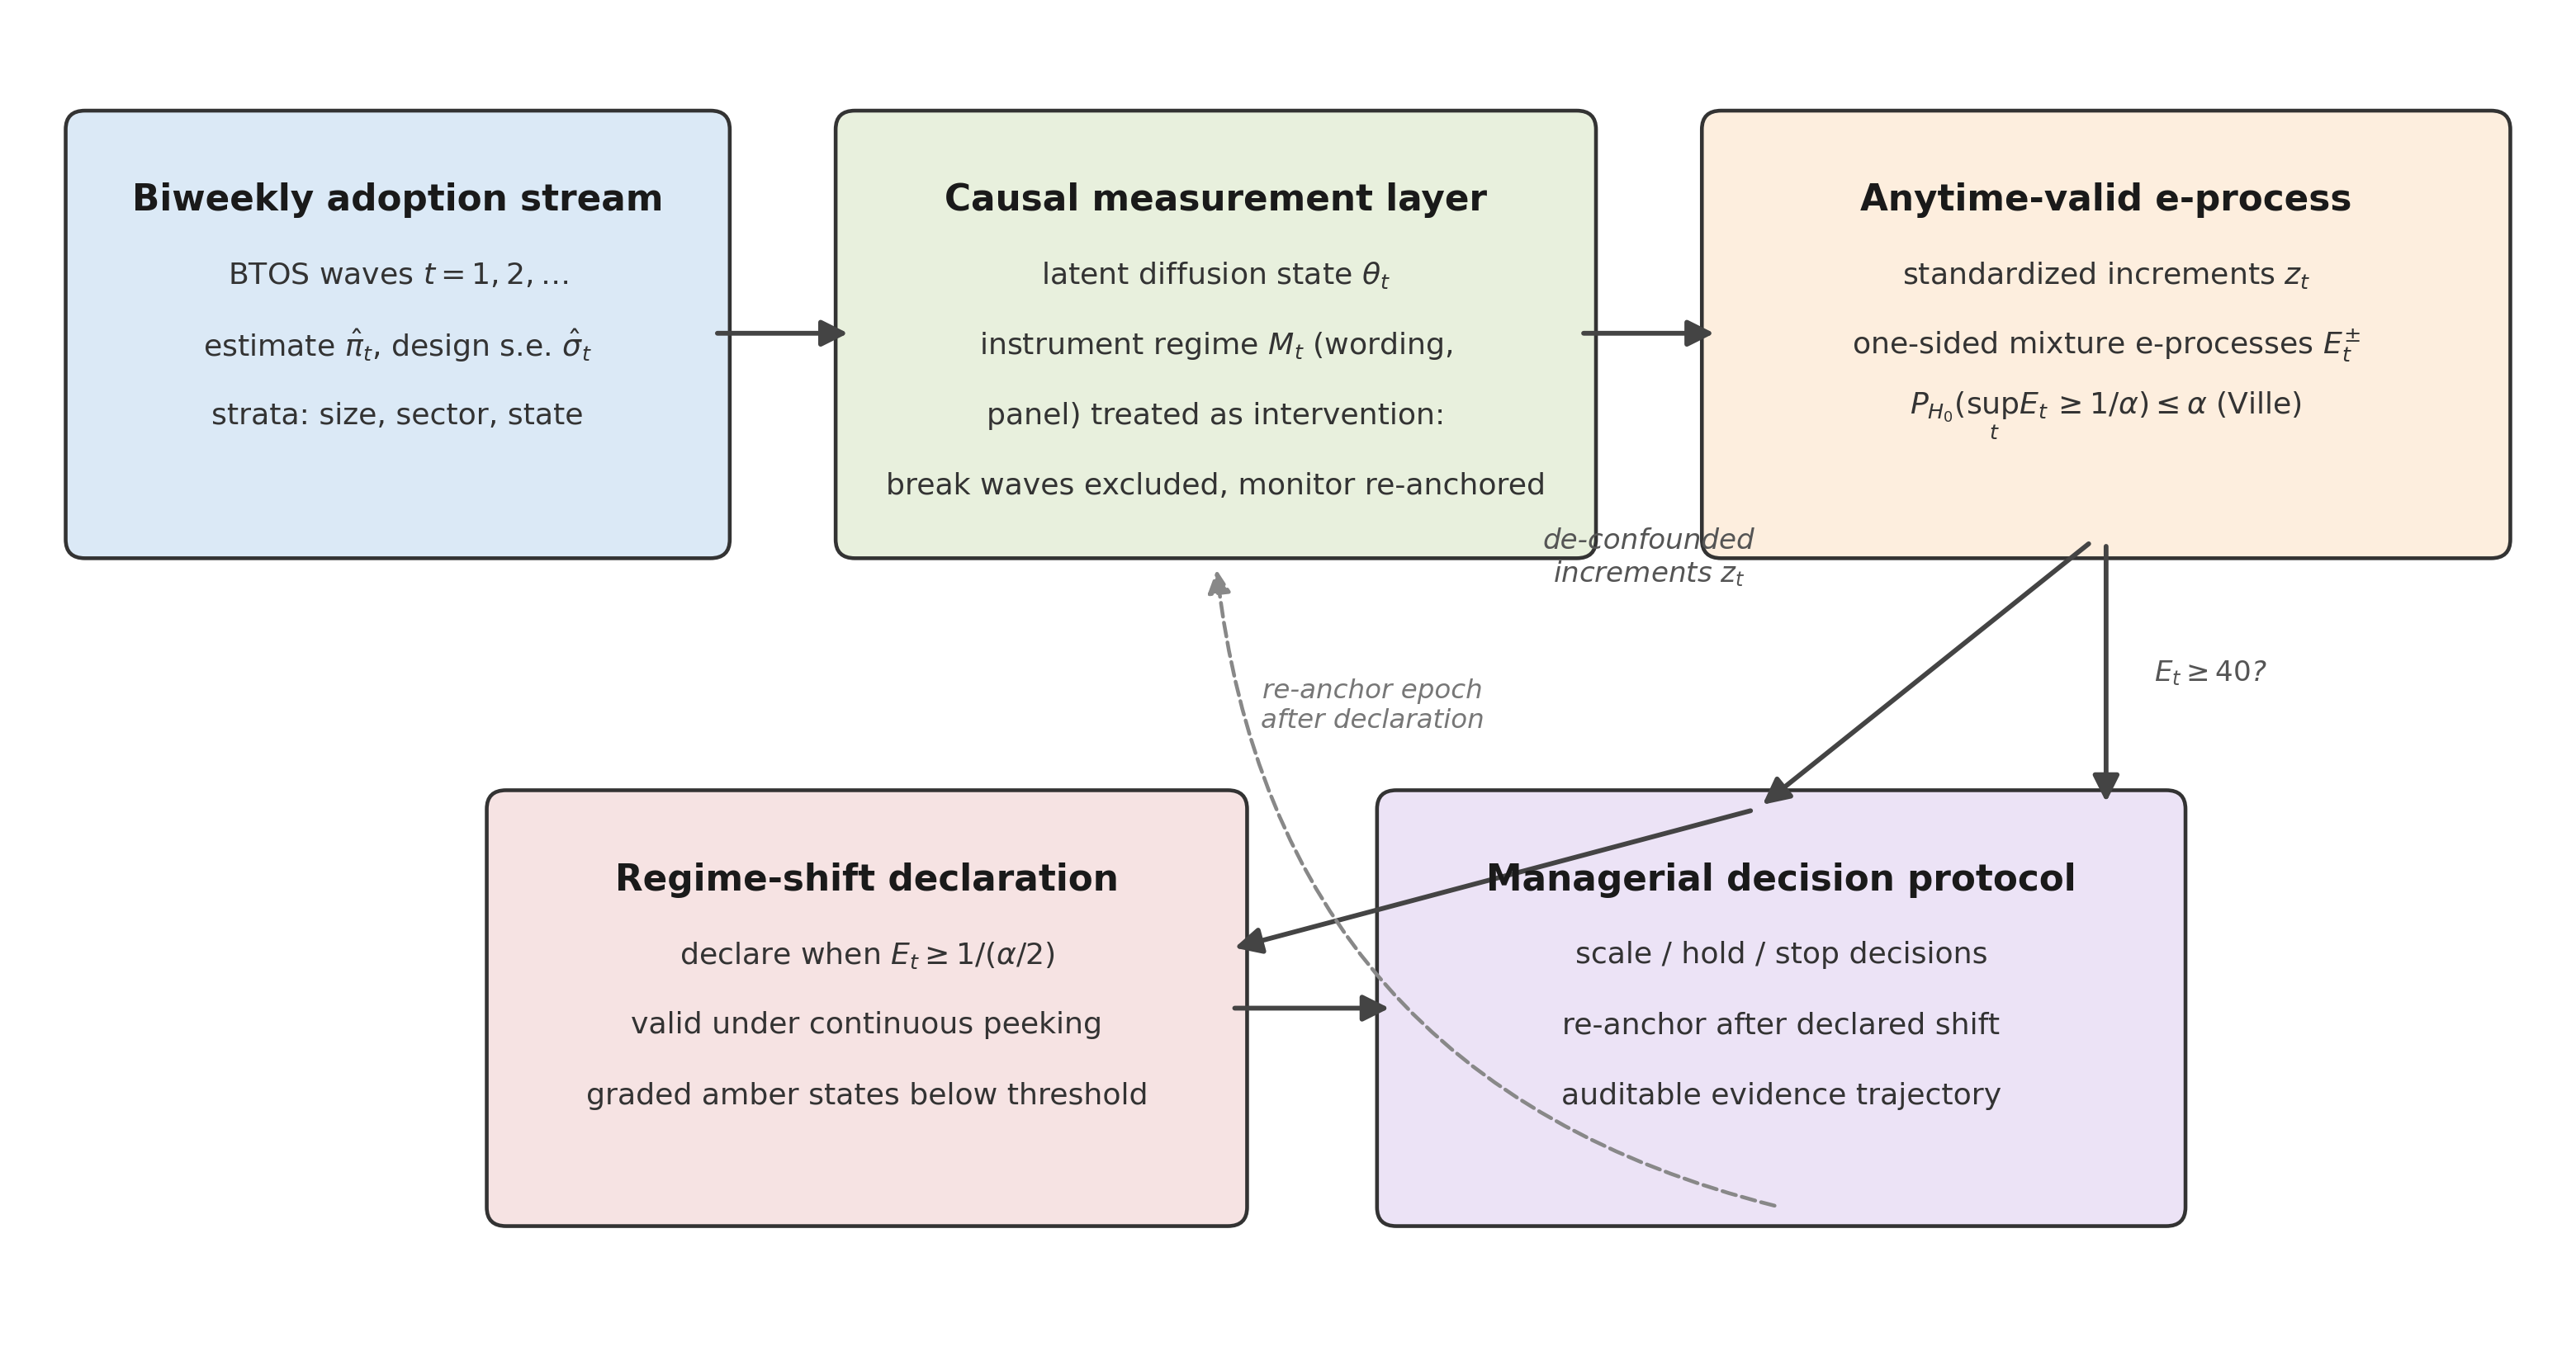
\includegraphics[width=\textwidth]{figure1.png}
\caption{The causal e-process monitoring framework. The measurement layer separates the latent diffusion state $\theta_t$ from the instrument regime $M_t$; one-sided mixture e-processes accumulate time-uniformly valid evidence on standardized within-regime increments; declared shifts and instrument changes trigger re-anchoring.}
\label{fig:framework}
\end{figure}

\subsection{Observation model and null hypotheses}
\label{sec:model}

Let $t = 1, 2, \dots$ index biweekly survey waves within a measurement regime. The published series delivers a weighted adoption-rate estimate $\hat{\pi}_t$ (percent of businesses reporting AI use in the past two weeks) with design-based standard error $\hat{\sigma}_t$, together with parallel series for planned adoption and for strata $k = 1, \dots, K$ (employment-size classes, sectors, states). We posit a latent diffusion state $\theta_t$---the population adoption propensity under a fixed, ideal instrument---and a measurement regime $M_t$ recording the active question wording and panel design. The observation equation is
\begin{equation}
\hat{\pi}_t \;=\; g(\theta_t, M_t) + \varepsilon_t, \qquad \varepsilon_t \mid \mathcal{F}_{t-1} \sim \mathcal{N}(0, \hat{\sigma}_t^2),
\label{eq:obs}
\end{equation}
where $g$ maps the latent state through the instrument (a narrower wording truncates $\theta_t$ to its production-function component) and the Gaussian approximation for the sampling error $\varepsilon_t$ is justified by the survey's scale: each biweekly estimate aggregates roughly 15,000--20,000 weighted responses \citep{fed2026}, and consecutive waves are drawn from different rotation panels, so sampling errors are independent across waves. Instrument redesigns are interventions $\mathrm{do}(M_t = m')$ on the observation process: they change $g$, not $\theta_t$. The monitoring question is whether $\theta_t$ has departed from a baseline path---not whether $\hat{\pi}_t$ has jumped.

Within a regime, define the increment $\Delta_t = \hat{\pi}_t - \hat{\pi}_{t-1}$. A surveillance epoch $e$ is endowed with a \emph{baseline slope} $\beta_e$ (percentage points per wave), fixed at the epoch's start from information available at that time. The epoch's null hypothesis is that the latent path continues at the baseline rate:
\begin{equation}
H_0^{(e)}:\quad \E[\Delta_t \mid \mathcal{F}_{t-1}] = \beta_e
\quad\text{with}\quad
\Delta_t - \beta_e \sim \mathcal{N}(0, \sigma_t^2),
\qquad
\sigma_t^2 = \hat{\sigma}_t^2 + \hat{\sigma}_{t-1}^2 + \mathrm{se}(\hat{\beta}_e)^2,
\label{eq:null}
\end{equation}
where $\mathrm{se}(\hat{\beta}_e)$ accounts for estimation error in an anchored slope (zero when $\beta_e$ is pre-registered rather than estimated). Under $H_0^{(e)}$ the standardized increments $z_t = (\Delta_t - \beta_e)/\sigma_t$ are independent standard normal. Rejecting $H_0^{(e)}$ upward is evidence of takeoff or acceleration relative to the baseline; rejecting downward is evidence of deceleration or stagnation. The null is deliberately sharp: it attributes all within-regime dispersion to sampling error, so that \emph{any} persistent movement of the latent path away from the baseline counts as signal. Section~\ref{sec:robust} examines robustness to relaxing this attribution.

\subsection{One-sided mixture e-processes}
\label{sec:eprocess}

For each epoch we run two one-sided monitors built from Robbins's method of mixtures \citep{robbins1970}. Let $S_n = \sum_{s=1}^{n} z_s$ denote the cumulative standardized evidence after $n$ within-epoch increments and let $\tau > 0$ be a prior scale. Mixing the Gaussian likelihood ratio $\exp(\delta S_n - n\delta^2/2)$ over a half-normal prior on the drift $\delta > 0$ gives, in closed form (derivation in \ref{app:derivation}),
\begin{equation}
E_n^{+} \;=\; \frac{2}{\tau\sqrt{a_n}}\;\Phi\!\left(\frac{S_n}{\sqrt{a_n}}\right)\exp\!\left(\frac{S_n^2}{2 a_n}\right),
\qquad a_n = n + \tau^{-2},
\label{eq:evalue}
\end{equation}
with $E_0^{+} = 1$, and symmetrically $E_n^{-}$ obtained by replacing $S_n$ with $-S_n$. Under $H_0^{(e)}$, $(E_n^{+})$ and $(E_n^{-})$ are nonnegative martingales with initial value one; more generally, under the composite one-sided null $\E[z_t \mid \mathcal{F}_{t-1}] \le 0$ (with unit-variance Gaussian noise), $(E_n^{+})$ is a supermartingale (\ref{app:derivation}). Ville's inequality therefore gives the time-uniform guarantee
\begin{equation}
\Prob_{H_0}\!\left(\exists\, n:\; E_n^{+} \ge \tfrac{1}{\alpha/2}\right) \le \tfrac{\alpha}{2},
\label{eq:ville}
\end{equation}
and likewise for $E_n^{-}$, so that declaring a regime shift the first time \emph{either} monitor reaches $1/(\alpha/2) = 40$ (at $\alpha = 0.05$) controls the per-epoch false-declaration probability at $\alpha$ no matter how often the series is inspected or when monitoring stops. Throughout we set $\tau = 1$, a unit prior scale on the standardized drift; Section~\ref{sec:robust} shows the results are insensitive to this choice. Because $E_n$ is a likelihood-ratio-type quantity, intermediate values carry graded meaning---$E_n = 10$ is 10-to-1 evidence against the baseline---which motivates the ``amber'' states of the decision protocol below, an interpretive resource that repeated $p$-values cannot supply under continuous monitoring.

\subsection{Surveillance epochs and re-anchoring}
\label{sec:epochs}

Monitoring proceeds through epochs, in the restart spirit of CUSUM \citep{page1954} and its e-process descendants \citep{shin2023}:

\begin{enumerate}
\item \textbf{Epoch 1 (takeoff surveillance).} The baseline slope is pre-registered at $\beta_1 = 0$: the null is that the latent adoption path is flat. Both one-sided monitors run from the first increment.
\item \textbf{Declaration.} The first time $E_n^{+} \ge 40$ or $E_n^{-} \ge 40$, a regime shift is declared with its direction, date, and terminal e-value recorded.
\item \textbf{Re-anchoring.} The next epoch's baseline slope $\hat{\beta}_{e+1}$ and its standard error are estimated by weighted least squares (weights $1/\hat{\sigma}_t^2$) on the $w = 8$ waves ending at the declaration wave---a window that uses only past data, so predictability and hence the supermartingale property are preserved. The new epoch begins at the following wave with fresh monitors at wealth one.
\item \textbf{Instrument interventions.} At a pre-announced redesign wave ($M_t \neq M_{t-1}$), the transition increment is excluded from every monitor---the do-operator made operational---and the monitor re-anchors on post-redesign waves once $w$ of them have accumulated. For discontinuities that are \emph{not} pre-announced, a cross-strata diagnostic (Section~\ref{sec:diagnostic}) allocates the wave to the measurement layer or the diffusion layer before any evidence is booked.
\end{enumerate}

\subsection{Cross-strata attribution diagnostic}
\label{sec:diagnostic}

Let $z_{k,t}$ be the standardized increment in stratum $k$ at wave $t$. The diagnostic compares the profile of a candidate break wave against the stratum's own within-regime history: an instrument event exhibits (i) synchronization---every stratum jumps in the same wave; (ii) extremity---each stratum's $|z_{k,t}|$ far exceeds the upper tail (we report the 95th percentile) of its within-regime $|z|$ distribution; and (iii) sign coherence consistent with the mechanical effect of the instrument change (a broader wording can only raise measured adoption). A genuine diffusion shift, by contrast, builds over multiple waves with magnitudes inside or near the within-regime tail and loads heterogeneously on strata according to exposure. The diagnostic is a screening rule with a causal-invariance rationale \citep{peters2016,rothenhausler2021} rather than a formally identified estimator; in the application it is unambiguous (Section~\ref{sec:break}).

\subsection{Retrospective surveillance with plug-in variance}
\label{sec:plugin}

The BTOS application enjoys a luxury most diffusion series lack: published design-based standard errors that make the sampling distribution of increments known. To extend surveillance to historical series without such metadata (Section~\ref{sec:longdata}), we replace $\sigma_t$ in \eqref{eq:null} with a \emph{predictable plug-in} scale: $\hat{\sigma}_t = \max\{\phi,\ 1.4826 \cdot \mathrm{MAD}(r_{t-W}, \dots, r_{t-1})\}$, the median-absolute-deviation estimate over the trailing $W = 8$ within-epoch increment residuals $r_s = \Delta_s - \beta_e$, seeded at each re-anchoring from the anchoring window's own residuals and floored at a series-specific constant $\phi$ chosen conservatively (0.8 percentage points per year for the annual internet series; 0.08 points per quarter for the quarterly e-commerce series). Because the scale at wave $t$ uses only information through $t-1$, predictability---and hence the supermartingale structure---is preserved mechanically; but the Gaussian null in \eqref{eq:null} now carries an estimated rather than known variance, so the time-uniform guarantee \eqref{eq:ville} holds only approximately. We therefore treat the retrospective results as an illustrative application of the surveillance logic, report e-values above $10^4$ simply as decisive, and reserve exact error statements for the design-based BTOS case.

\subsection{Decision protocol}
\label{sec:protocol}

Table~\ref{tab:protocol} maps monitor states to actions, separating \emph{statistical} thresholds (fixed by $\alpha$ and the e-process) from \emph{managerial} ones (encoding the asymmetry of scaling too early versus too late, and settable per organization).

\begin{table}[t]
\centering
\caption{Decision protocol linking e-process states to managerial actions ($\alpha = 0.05$; declaration threshold $1/(\alpha/2) = 40$ per one-sided monitor).}
\label{tab:protocol}
\small
\begin{tabular}{p{3.4cm}p{2.5cm}p{4.2cm}p{4.0cm}}
\toprule
Monitor state & Evidence level & Interpretation & Illustrative action \\
\midrule
$E_n < 2$ & Negligible & No credible departure from baseline path & Continue routine monitoring \\
$2 \le E_n < 10$ & Amber & Suggestive evidence; odds 2--10\,:\,1 against baseline & Prepare contingency; increase review cadence \\
$10 \le E_n < 40$ & Strong amber & Odds 10--40\,:\,1; declaration plausible soon & Pre-position decision; brief stakeholders \\
$E_n \ge 40$ & Declared shift & Time-uniformly valid rejection at level $\alpha$ & Execute scale/hold/stop decision; re-anchor monitor \\
Instrument change ($M_t \neq M_{t-1}$) & --- & Measurement intervention, not diffusion evidence & Exclude wave; re-baseline; document break \\
\bottomrule
\end{tabular}
\end{table}

\subsection{Comparators}
\label{sec:comparators}

Three baselines represent current monitoring practice, each applied at every release to the naively spliced series (legacy waves followed by revised-wording waves, as a dashboard unaware of the redesign would splice them): (a) a repeated two-sample $z$-test comparing the latest four waves with the preceding four, using the design-based standard errors, uncorrected at the 5\% level; (b) the same with a Bonferroni correction over the number of looks made so far; and (c) a moving-average crossing rule (3-wave minus 8-wave means changing sign), the de facto dashboard heuristic. For each we record the first alarm, the number of alarm waves and of distinct alarm episodes over the 48 possible looks, and behavior at the November 2025 redesign.

\section{Data}
\label{sec:data}

\subsection{The Business Trends and Outlook Survey, 2023--2025}
\label{sec:btosdata}

The BTOS is an experimental data product of the U.S.\ Census Bureau designed to measure business conditions at high frequency. The sample comprises approximately 1.2 million nonfarm employer businesses divided into six rotating panels of roughly 200,000; each panel reports once every twelve weeks over a year, and collection occurs every two weeks, yielding a continuous biweekly national series \citep{censusmethod2025,census2026pr}. Estimates are weighted to be representative at the national, state, sector, and employment-size levels; the average biweekly response rate over the AI-content period is about 16 percent \citep{bonney2024}, and estimates failing publication standards are suppressed.

Two core AI questions have run since the collection period beginning 11 September 2023 \citep{bonney2024}. From September 2023 through October 2025 the current-use question read: \emph{``In the last two weeks, did this business use Artificial Intelligence (AI) in producing goods or services? (Examples of AI: machine learning, natural language processing, virtual agents, voice recognition, etc.)''} Beginning with the collection of 17 November 2025, ``in producing goods or services'' was replaced by ``in any of its business functions,'' and a supplement fielded from 17 November 2025 to 8 February 2026 added detail on adoption across fifteen business functions \citep{census2026pr}. A companion question asks about expected AI use over the next six months under the same wordings.

Our analysis dataset consists of every published national and employment-size-class estimate of the two AI questions, with design-based standard errors, from the survey's public data downloads. Because the Census Bureau's file of 15 December 2025 removed the legacy-wording AI rows when introducing the revised series, we splice two archived vintages of the official National and Employment Size Class files---downloaded 8 December 2025 (which retains the full legacy series) and 15 December 2025 (which carries the revised series)---following the vintage documentation of \citet{goldschlag2025}. The result is 56 national waves: 54 legacy-wording waves covering collection periods ending 24 September 2023 through 5 October 2025 (periods 202319--202520), and two revised-wording waves ending 30 November and 14 December 2025 (202524--202525). No AI estimates were published for the three transition periods 202521--202523. National design-based standard errors have median 0.15 percentage points (range 0.08--0.23); size-class standard errors are larger, with medians from 0.23 (1--4 employees) to 1.21 (250+ employees) percentage points. The exact analysis dataset (two CSV files) and replication code accompany the manuscript.

The headline contours of the series are as follows. Under the legacy wording, national current use rose from 3.7 percent (24 September 2023) to 4.9 percent by end-2023, slipped to 4.7 percent by 30 June 2024, resumed growth to 6.3 percent by 29 December 2024, accelerated to 8.3 percent by 20 April 2025, flattened near 8.8 percent through 10 August 2025, and closed the legacy period at 10.0 percent on 5 October 2025. Planned use ran above current use throughout, from 6.3 to 14.0 percent. Under the revised wording, current use printed 17.3 and 17.2 percent and planned use 21.1 and 20.9 percent in the two available waves---consistent with subsequently published Census reporting that the broadened measure hovered between 17 and 20 percent into 2026 \citep{censusstory2026}.

\subsection{Long-run diffusion series, 1990--2026}
\label{sec:longdata}

Two public series extend the surveillance horizon to three and a half decades. \emph{Internet users as a share of the U.S.\ population}, annual, 1990--2024, from the International Telecommunication Union's World Telecommunication/ICT Indicators database as disseminated by the World Bank (indicator IT.NET.USER.ZS) and retrieved from FRED \citep{fredinternet}: the series rises from 0.79 percent in 1990 to 94.7 percent in 2024, tracing the canonical S-curve of a saturating general-purpose technology. It splices household-survey estimates with ITU and World Bank estimation methods, so---unlike the BTOS---it carries neither design-based standard errors nor strata, and it contains a conspicuous single-year discontinuity of $+10.9$ points between 2015 and 2016 following a decade in which measured penetration fluctuated between 69 and 75 percent. \emph{E-commerce sales as a share of total U.S.\ retail sales}, quarterly and seasonally adjusted, 1999Q4--2026Q1, from the Census Bureau's Quarterly Retail E-Commerce Sales program retrieved from FRED \citep{fredecom}: 106 quarters from 0.6 to 16.9 percent, including the celebrated COVID-19 jump (11.9 to 16.3 percent between 2020Q1 and 2020Q2), the 2021--2022 partial reversal to 14.2 percent, and renewed growth thereafter. Both extracts are included verbatim in the supplementary data.

\section{Results}
\label{sec:results}

\begin{figure}[t]
\centering
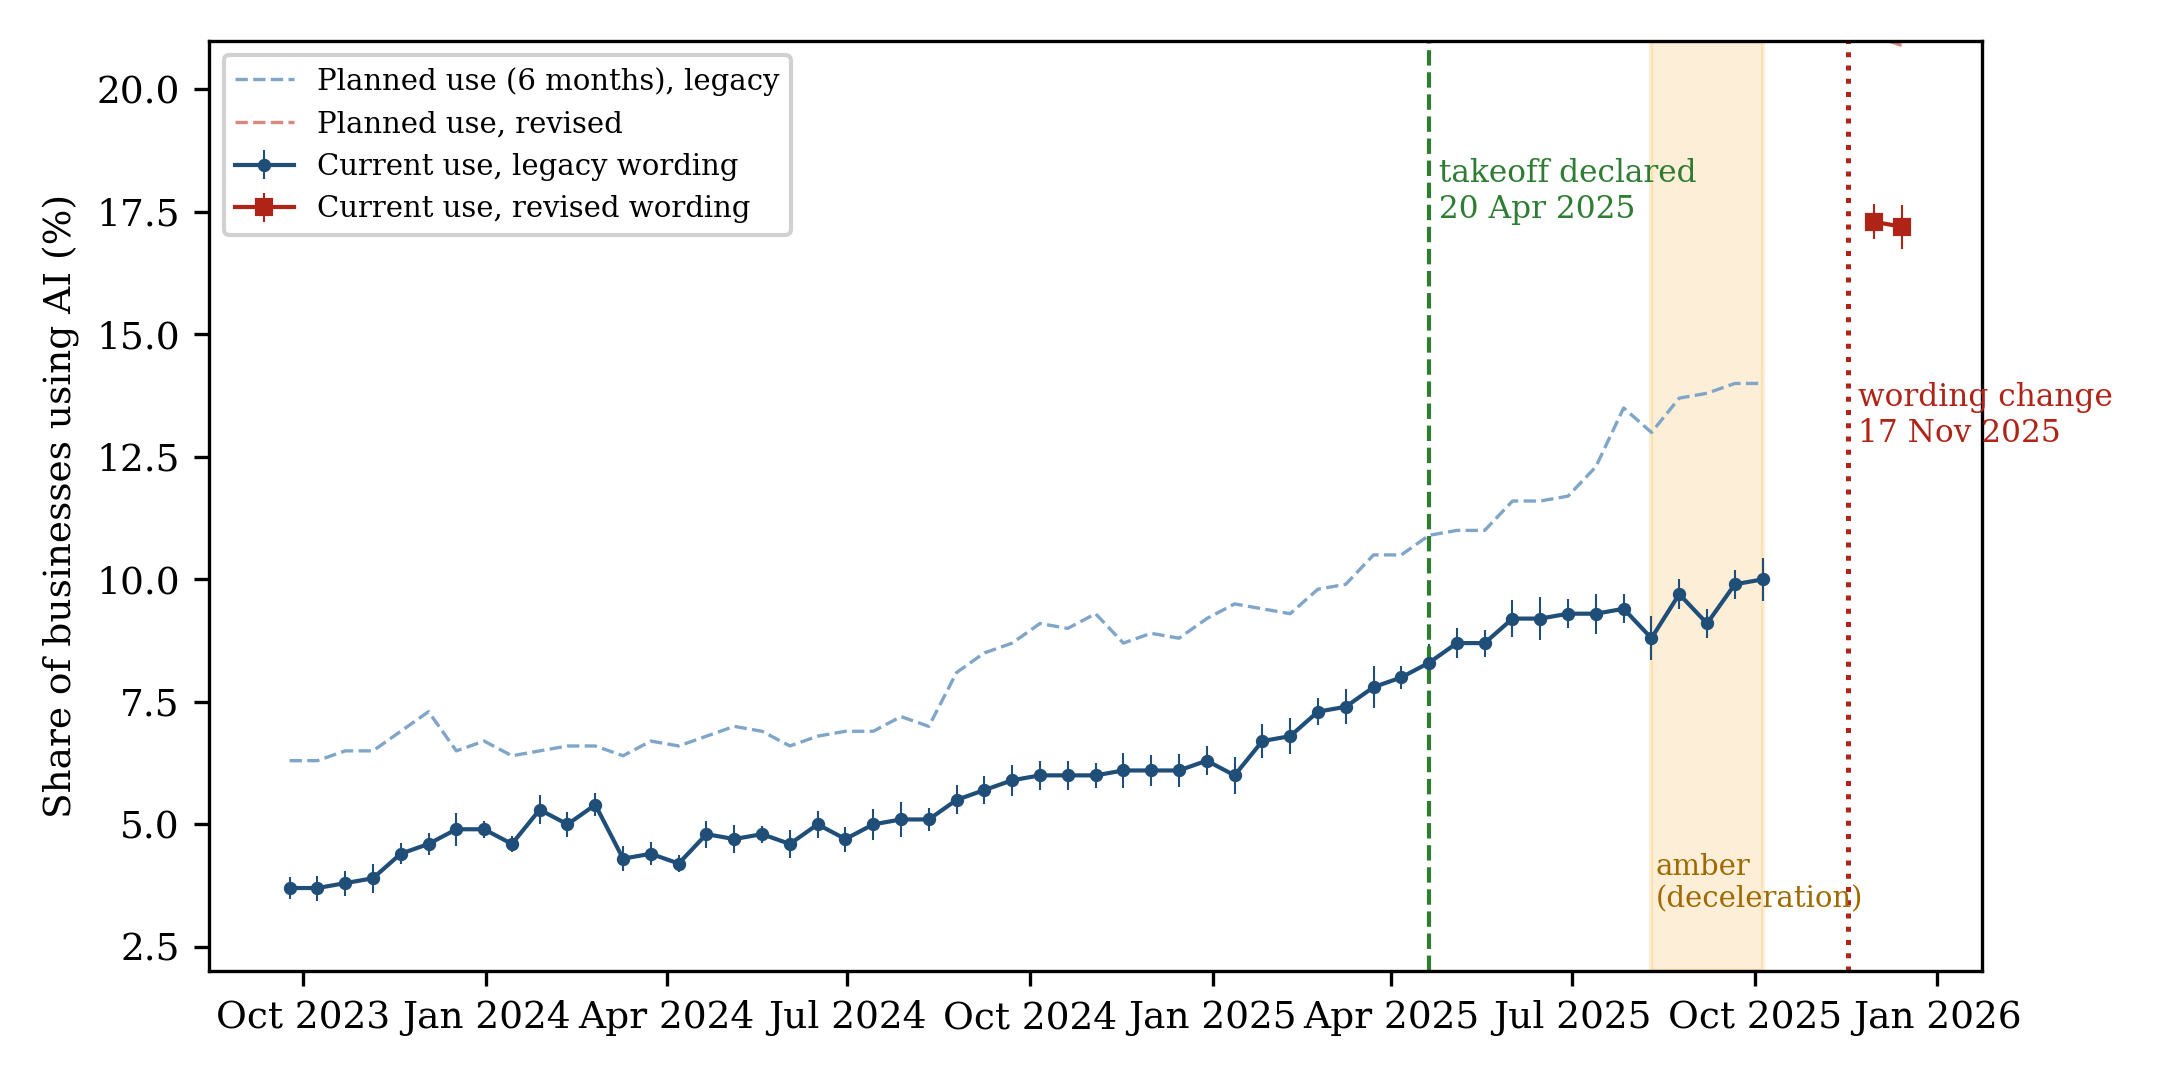
\includegraphics[width=\textwidth]{figure2.png}
\caption{The BTOS national AI adoption series, September 2023--December 2025, with monitoring outcomes. Solid lines with 95\% intervals show current use under the legacy (blue circles) and revised (red squares) wordings; dashed lines show planned use over the next six months. The green dashed line marks the takeoff declaration (20 April 2025); the shaded band marks the span during which the deceleration monitor held amber-or-higher evidence (10 August--5 October 2025); the red dotted line marks the question-wording intervention (17 November 2025). No AI estimates were published for the three transition periods between 5 October and 30 November 2025. Source: authors' calculations from U.S.\ Census Bureau BTOS public data.}
\label{fig:series}
\end{figure}

\begin{figure}[t]
\centering
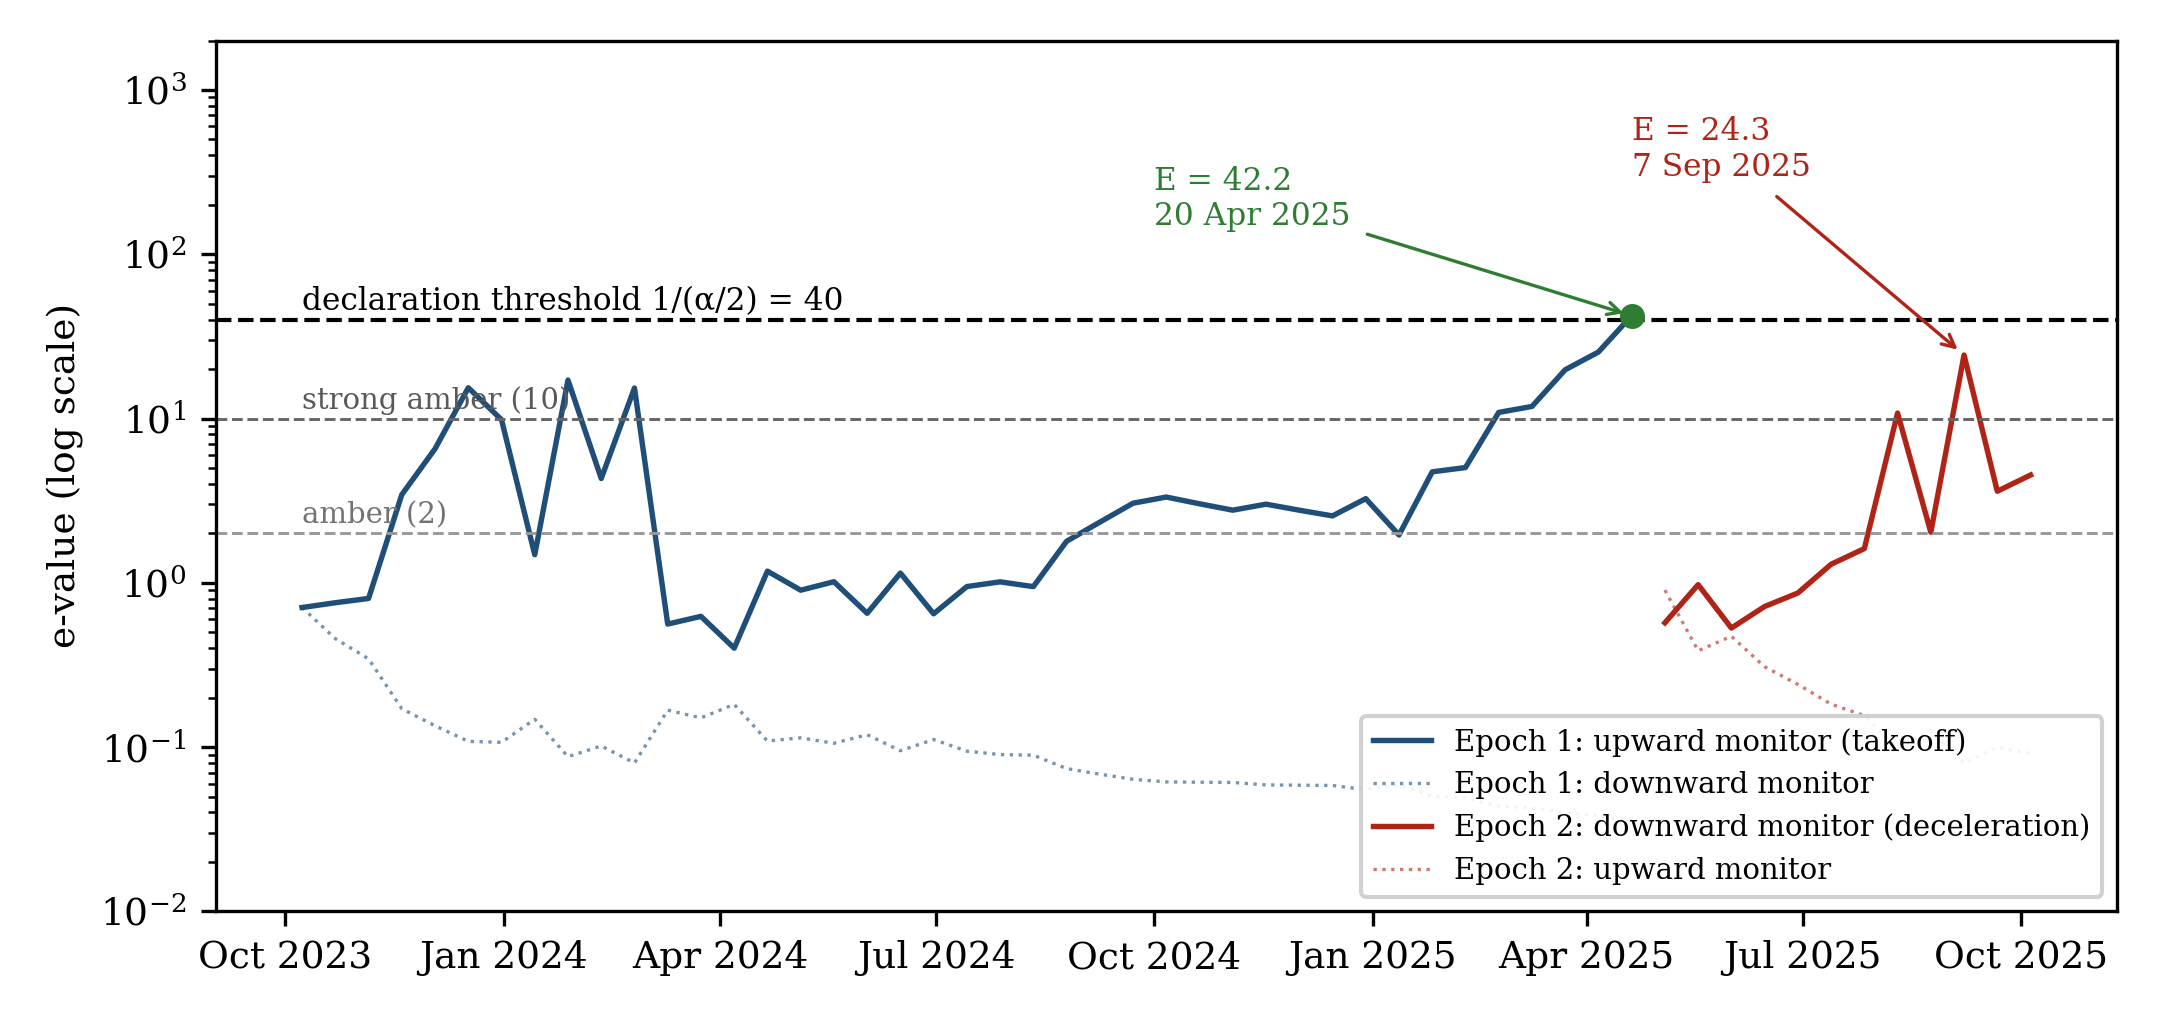
\includegraphics[width=\textwidth]{figure3.png}
\caption{E-value trajectories of the national monitors (log scale). Epoch 1 tests the pre-registered flat baseline ($\beta_1 = 0$); Epoch 2 tests the anchored early-2025 growth rate ($\hat{\beta}_2 = 0.299 \pm 0.027$ pp per wave, estimated on the eight waves ending at the declaration). The upward monitor crosses the declaration threshold of 40 on 20 April 2025 ($E = 42.2$); the Epoch-2 downward monitor peaks at $E = 24.3$ on 7 September 2025 without crossing.}
\label{fig:evalues}
\end{figure}

\subsection{Episode 1: the takeoff and its declaration (RQ1, RQ3)}
\label{sec:takeoff}

Figures~\ref{fig:series} and \ref{fig:evalues} display the series and the monitors' evidence trajectories. Epoch 1 opens at the second published wave (8 October 2023) against the pre-registered flat baseline. Evidence accumulates quickly through the late-2023 growth spurt: the upward monitor passes the amber threshold ($E \ge 2$) on 19 November 2023, passes 10 on 17 December 2023 ($E = 15.4$), and reaches a local peak of 17.1 on 28 January 2024. It then does something a $p$-value stream cannot do: it retreats. As measured adoption stalls through the first half of 2024 (4.9 percent at end-2023 to 4.7 percent on 30 June 2024), the negative increments consume accumulated wealth, and the monitor bottoms at $E = 0.4$ on 7 April 2024---the evidence for a takeoff, evaluated against the full history, had genuinely weakened. The monitor rebuilds through the second-half-2024 recovery (6.3 percent by 29 December 2024) and the early-2025 acceleration (6.0 percent on 12 January to 8.3 percent on 20 April 2025), and crosses the declaration threshold on \textbf{20 April 2025} with terminal e-value \textbf{42.2}, after 41 monitored increments. By Ville's inequality \eqref{eq:ville}, the probability that a flat latent path would ever have produced such a crossing is at most 2.5 percent, no matter how many times the series was inspected along the way.

The declaration date is informative rather than embarrassing. The monitor did not certify a takeoff during the 2023 spurt because, at that point, a flat path punctuated by a transient could not yet be excluded at the stated error rate---and the first half of 2024 showed exactly such a stall. The declaration arrives precisely when the acceleration becomes sustained. The answer to RQ1 is therefore affirmative in a specific sense: real-time detection with time-uniform guarantees is feasible on official high-frequency adoption data, and the guarantee's price is measured restraint during ambiguous phases, not blindness.

\subsection{Episode 2: the mid-2025 deceleration as graded evidence (RQ3)}
\label{sec:deceleration}

Upon declaration, the monitor re-anchors: weighted least squares on the eight waves ending at the declaration (12 January--20 April 2025) fixes the Epoch-2 baseline at $\hat{\beta}_2 = 0.299 \pm 0.027$ percentage points per wave---the null that the early-2025 growth tempo continues. Epoch 2 opens on 4 May 2025. Against this demanding baseline, the flattening of the series through the summer (8.3 percent in April to 8.8 percent on 10 August 2025) drives the \emph{downward} monitor upward: it reaches amber on 10 August 2025, and peaks at $E = 24.3$ on 7 September 2025---24-to-1 evidence that growth had fallen below the anchored tempo, within the strong-amber band of Table~\ref{tab:protocol} but short of declaration. The evidence then recedes to $E = 4.5$ by 5 October 2025 as growth resumes (9.9 and 10.0 percent in the final legacy waves). The upward monitor never exceeds 0.9 in Epoch 2.

Two readings of this episode matter for practice. First, the monitor \emph{quantified} the widely discussed 2025 deceleration in real time---at its peak, a manager consulting the dashboard would have seen 24-to-1 odds that AI diffusion momentum had broken---while correctly declining to certify a regime change that the subsequent data contradict: the series re-accelerated within weeks, and the revised-wording waves and later Census reporting show continued growth \citep{censusstory2026}. Had the organization operated at $\alpha = 0.10$ instead of $0.05$ (declaration threshold 20), a deceleration \emph{would} have been declared on 7 September 2025 and then contradicted---a concrete illustration of what the choice of $\alpha$ buys. Second, the moving-average heuristic run over the same episode crossed downward on 7 September and back upward on 21 September 2025 (Figure~\ref{fig:alarms}): a whipsaw delivering two contradictory signals fourteen days apart, with no statement of error probability attached to either.

\subsection{Episode 3: the November 2025 redesign as a measurement event (RQ2)}
\label{sec:break}

\begin{figure}[t]
\centering
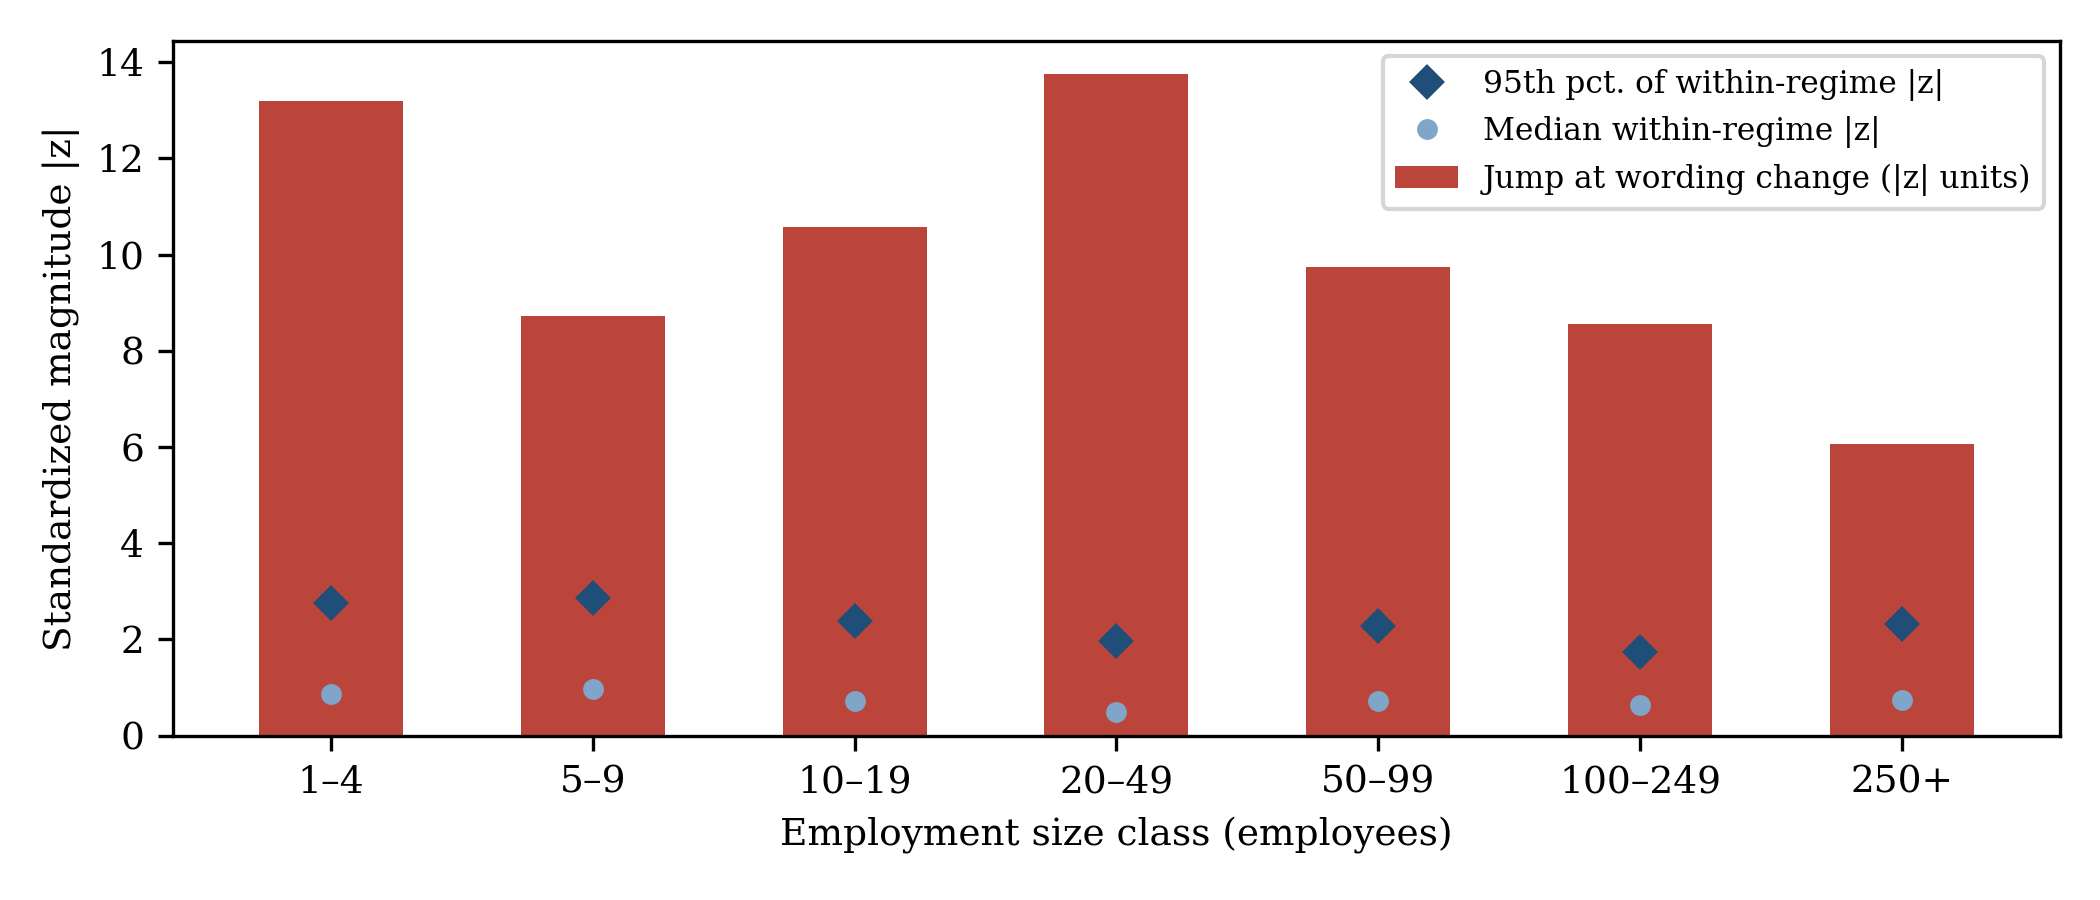
\includegraphics[width=0.95\textwidth]{figure5.png}
\caption{Cross-strata attribution diagnostic at the 17 November 2025 wording change. Bars show each employment-size class's jump between its last legacy-wording and first revised-wording estimate, in units of the combined design-based standard error; markers show the median and 95th percentile of that class's within-regime standardized wave-to-wave movements. Every class jumps simultaneously, by 2--7 times its within-regime 95th percentile, with a common sign---the signature of an instrument intervention, not of diffusion.}
\label{fig:strata}
\end{figure}

Between the last legacy wave (10.0 percent, 5 October 2025) and the first revised-wording wave (17.3 percent, 30 November 2025) the published series jumps 7.3 percentage points---25.7 combined standard errors, against a within-regime national history in which the median absolute standardized movement is 0.94 and the maximum is 6.2. Because the redesign was announced by the data provider, the causal layer excludes the transition increment by construction, and the monitor books no diffusion evidence from it. The cross-strata diagnostic of Section~\ref{sec:diagnostic}, applied as if the break had \emph{not} been announced, confirms the attribution decisively (Figure~\ref{fig:strata} and Table~\ref{tab:strata}): all seven employment-size classes jump in the same single wave, by 6.1 to 13.8 standard errors---between roughly 2.6 and 7.0 times their respective within-regime 95th percentiles (1.74--2.85)---and all in the same direction, as the mechanically broader wording implies. Nothing in the genuine takeoff resembles this signature: the takeoff built over more than a year, wave by wave, with movements inside or near the within-regime tail.

The contrast with conventional practice is stark. The naive rolling $z$-test, applied to the spliced series as a redesign-unaware dashboard would splice it, produces its largest statistic of the entire sample at the break ($|z| = 32.9$) and alarms there under both the uncorrected and Bonferroni-corrected versions---certifying, at any conventional significance level, the largest ``diffusion shock'' on record where none occurred. The answer to RQ2 is that the separation is achievable and cheap: it requires only that the monitoring architecture carry the instrument regime as an explicit variable and treat its changes as interventions, with the cross-strata signature available as verification when provenance is uncertain.

\subsection{Comparison with conventional monitoring (RQ3)}
\label{sec:comparison}

\begin{figure}[t]
\centering
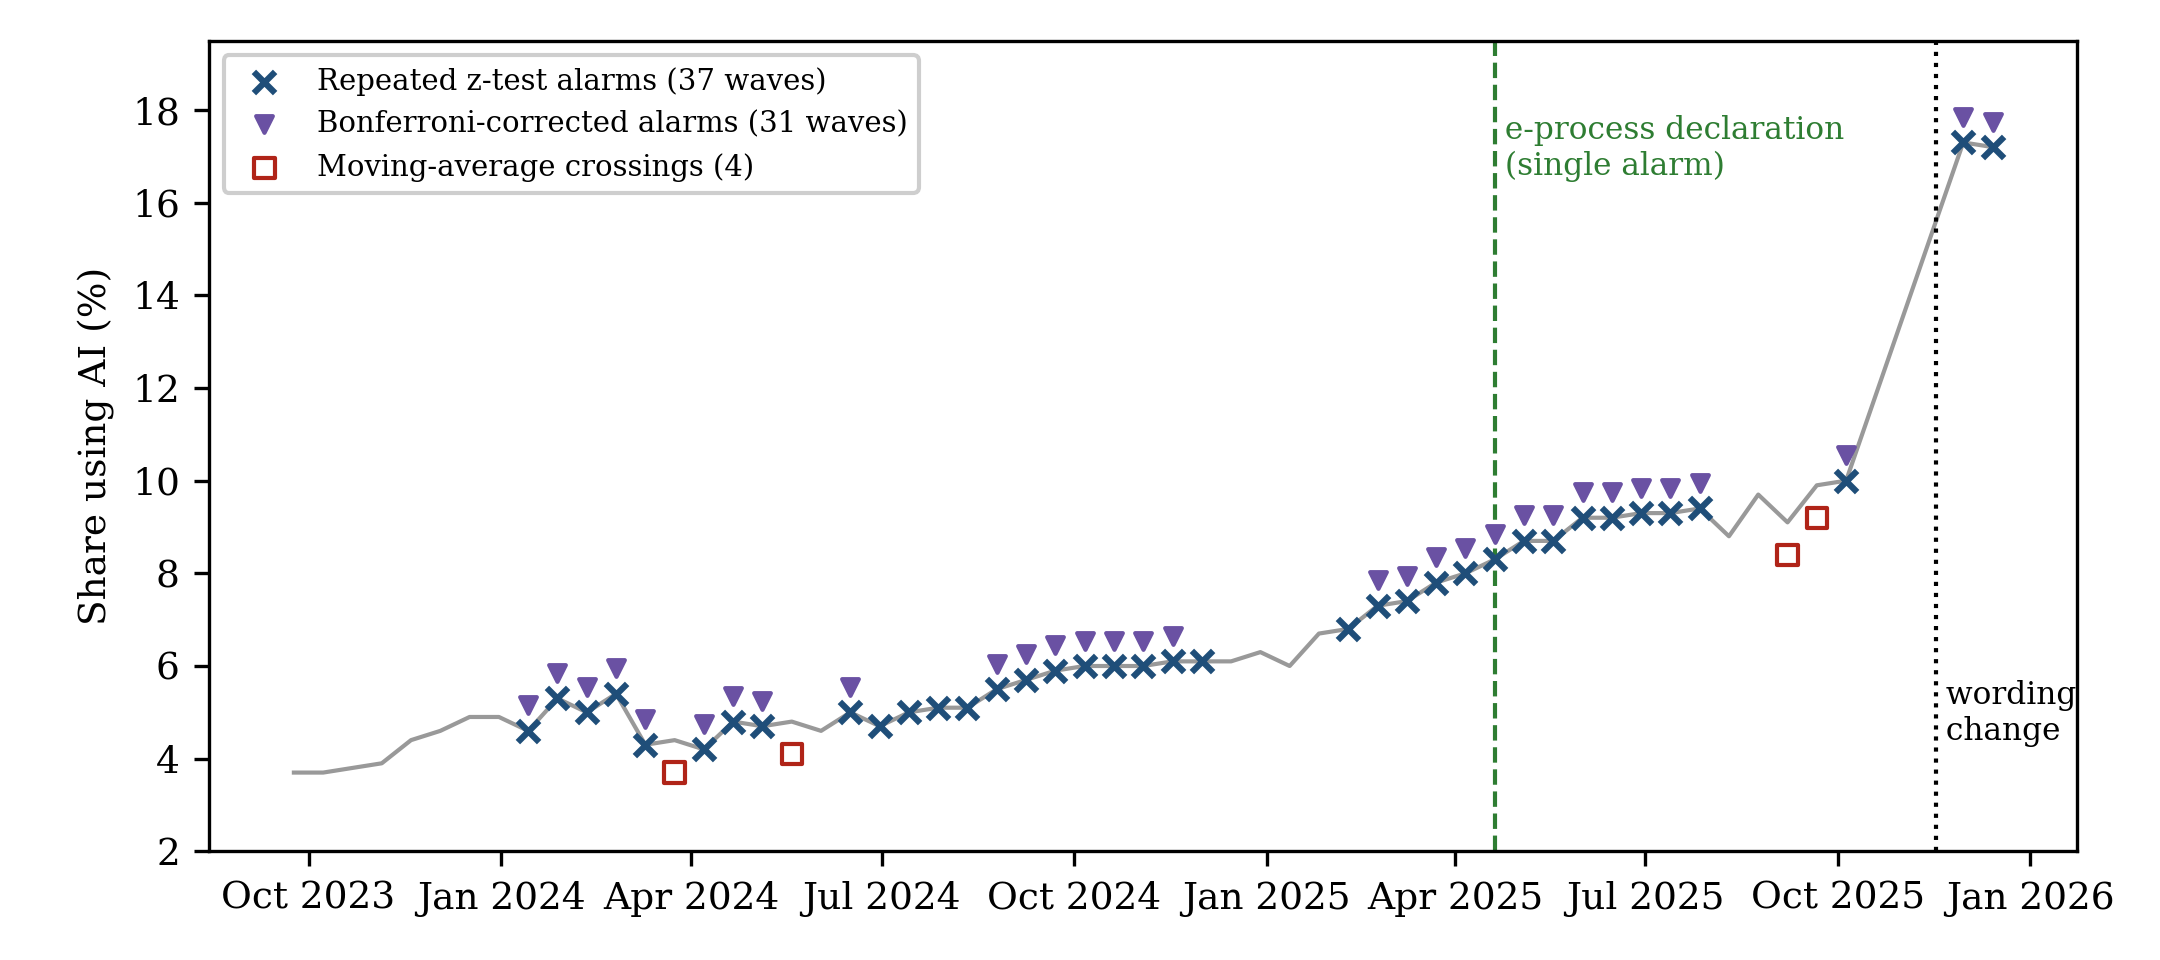
\includegraphics[width=\textwidth]{figure4.png}
\caption{Alarm behavior of conventional monitoring rules over the naively spliced series, September 2023--December 2025. Crosses: repeated four-versus-four-wave $z$-test, uncorrected (37 alarm waves of 48 looks). Triangles: the same with Bonferroni correction over looks (31 alarm waves). Open squares: 3-versus-8-wave moving-average crossings (four crossings, including the September 2025 whipsaw). The e-process framework produces a single declaration (green dashed line) and excludes the wording change (dotted line) by design.}
\label{fig:alarms}
\end{figure}

\begin{table}[t]
\centering
\caption{Detection and alarm behavior across monitoring methods on the BTOS national AI series (48 possible looks, September 2023--December 2025).}
\label{tab:methods}
\small
\begin{tabular}{lcccc}
\toprule
Method & First alarm & Alarm waves & Distinct episodes & Alarms at redesign \\
\midrule
Causal e-process ($\alpha=0.05$) & 20 Apr 2025$^{a}$ & 1 & 1 & 0 (excluded by design) \\
Repeated $z$-test, uncorrected & 14 Jan 2024 & 37 & 5 & yes ($|z| = 32.9$) \\
Repeated $z$-test, Bonferroni & 14 Jan 2024 & 31 & 6 & yes \\
Moving-average crossing (3, 8) & 24 Mar 2024 & 4 & 3 & no crossing \\
\bottomrule
\end{tabular}
\begin{minipage}{0.94\textwidth}
\vspace{2pt}
{\footnotesize $^{a}$Declaration with terminal e-value 42.2; graded evidence available continuously beforehand (amber from 19 November 2023, strong amber from 17 December 2023, trough 0.4 on 7 April 2024). Moving-average crossing dates: 24 March 2024, 19 May 2024, 7 September 2025, 21 September 2025.}
\end{minipage}
\end{table}

Table~\ref{tab:methods} and Figure~\ref{fig:alarms} summarize the comparison, and the honest reading cuts both ways. The repeated $z$-tests ``detect'' growth on 14 January 2024, fifteen months before the e-process declaration---but the same rule then alarms on 37 of 48 looks (31 after Bonferroni), including through the first-half-2024 stall and at the November 2025 redesign. A rule that is almost always alarming cannot date a regime change, cannot distinguish diffusion from measurement, and offers no interpretable error statement under open-ended monitoring: the uncorrected version's family-wise guarantee is void, and the Bonferroni version's guarantee, while formally valid look-by-look, is purchased by a level that shrinks toward zero as monitoring continues, with its 31 alarms demonstrating that in this high-precision setting the correction restrains nothing that matters. The moving-average rule is quiet by comparison but delivers whipsaws (two crossings in 2024 during the stall-recovery, two in September 2025) with no error control at all. The e-process trades earliness for validity and interpretability: one declaration, dated, with a terminal evidence ratio; a continuous graded evidence path before it; correct restraint during the plateau; and structural immunity to the instrument change. Which side of that trade a decision-maker should take depends on the cost of false regime declarations---and Section~\ref{sec:discussion} argues that for scaling decisions in technology management, those costs are high.

\subsection{Heterogeneity across firm-size classes}
\label{sec:strata}

\begin{table}[t]
\centering
\caption{Employment-size-class series and monitoring outcomes. ``Max $E^{+}$'' is the maximum of the takeoff (Epoch-1) upward monitor over the legacy period; no class reaches the declaration threshold of 40, reflecting larger stratum-level standard errors (median s.e.\ in percentage points shown). Jump columns give the movement between the last legacy-wording and first revised-wording estimates in percentage points and in combined standard errors, against the 95th percentile of within-regime standardized movements.}
\label{tab:strata}
\small
\begin{tabular}{lcccccccc}
\toprule
Size class & Sep 2023 & Oct 2025 & Nov 2025$^{r}$ & Med.\ s.e. & Max $E^{+}$ & Jump (pp) & Jump ($|z|$) & p95 within $|z|$ \\
\midrule
1--4       & 4.3 & 11.0 & 17.0 & 0.23 & 11.4 & 6.0  & 13.2 & 2.77 \\
5--9       & 3.0 &  8.6 & 15.5 & 0.29 &  4.0 & 6.9  &  8.7 & 2.85 \\
10--19     & 2.6 &  8.1 & 17.8 & 0.32 & 10.7 & 9.7  & 10.6 & 2.37 \\
20--49     & 2.6 &  7.0 & 18.7 & 0.36 &  1.8 & 11.7 & 13.8 & 1.96 \\
50--99     & 2.4 &  9.7 & 20.7 & 0.57 &  4.0 & 11.0 &  9.7 & 2.29 \\
100--249   & 2.5 &  8.8 & 23.7 & 0.92 &  1.3 & 14.9 &  8.6 & 1.74 \\
250+       & 3.1 & 13.0 & 30.5 & 1.21 & 12.9 & 17.5 &  6.1 & 2.31 \\
\bottomrule
\end{tabular}
\begin{minipage}{0.94\textwidth}
\vspace{2pt}
{\footnotesize Entries in percent of businesses except where noted. $^{r}$First revised-wording estimate (30 November 2025). Source: authors' calculations from U.S.\ Census Bureau BTOS public data (Employment Size Class files, vintages of 8 and 15 December 2025).}
\end{minipage}
\end{table}

Table~\ref{tab:strata} reports the size-class analysis. Levels replicate the familiar gradient---by the revised measure, adoption runs from 17.0 percent among the smallest firms to 30.5 percent among firms with 250 or more employees, and the revised-wording jump is largest in absolute terms for large firms (17.5 percentage points), whose multi-function operations the legacy wording most severely under-counted. Stratum-level monitors, facing standard errors four to eight times the national ones, accumulate takeoff evidence that peaks in amber territory (maximum $E^{+}$ of 11.4--12.9 for the smallest and largest classes, weaker in between) without any stratum-level declaration in-sample---a transparent illustration that the framework's detection power is governed by the precision of the stream it watches, and that national-level surveillance, which pools that precision, is where declarations are earned. For the attribution diagnostic, the strata are decisive in the other direction, as Section~\ref{sec:break} showed: it is exactly because every class jumps at once, far outside its own history, that the redesign is unmistakable as a measurement event.

\subsection{The long view: three diffusion waves, 1990--2026}
\label{sec:longview}

\begin{figure}[t]
\centering
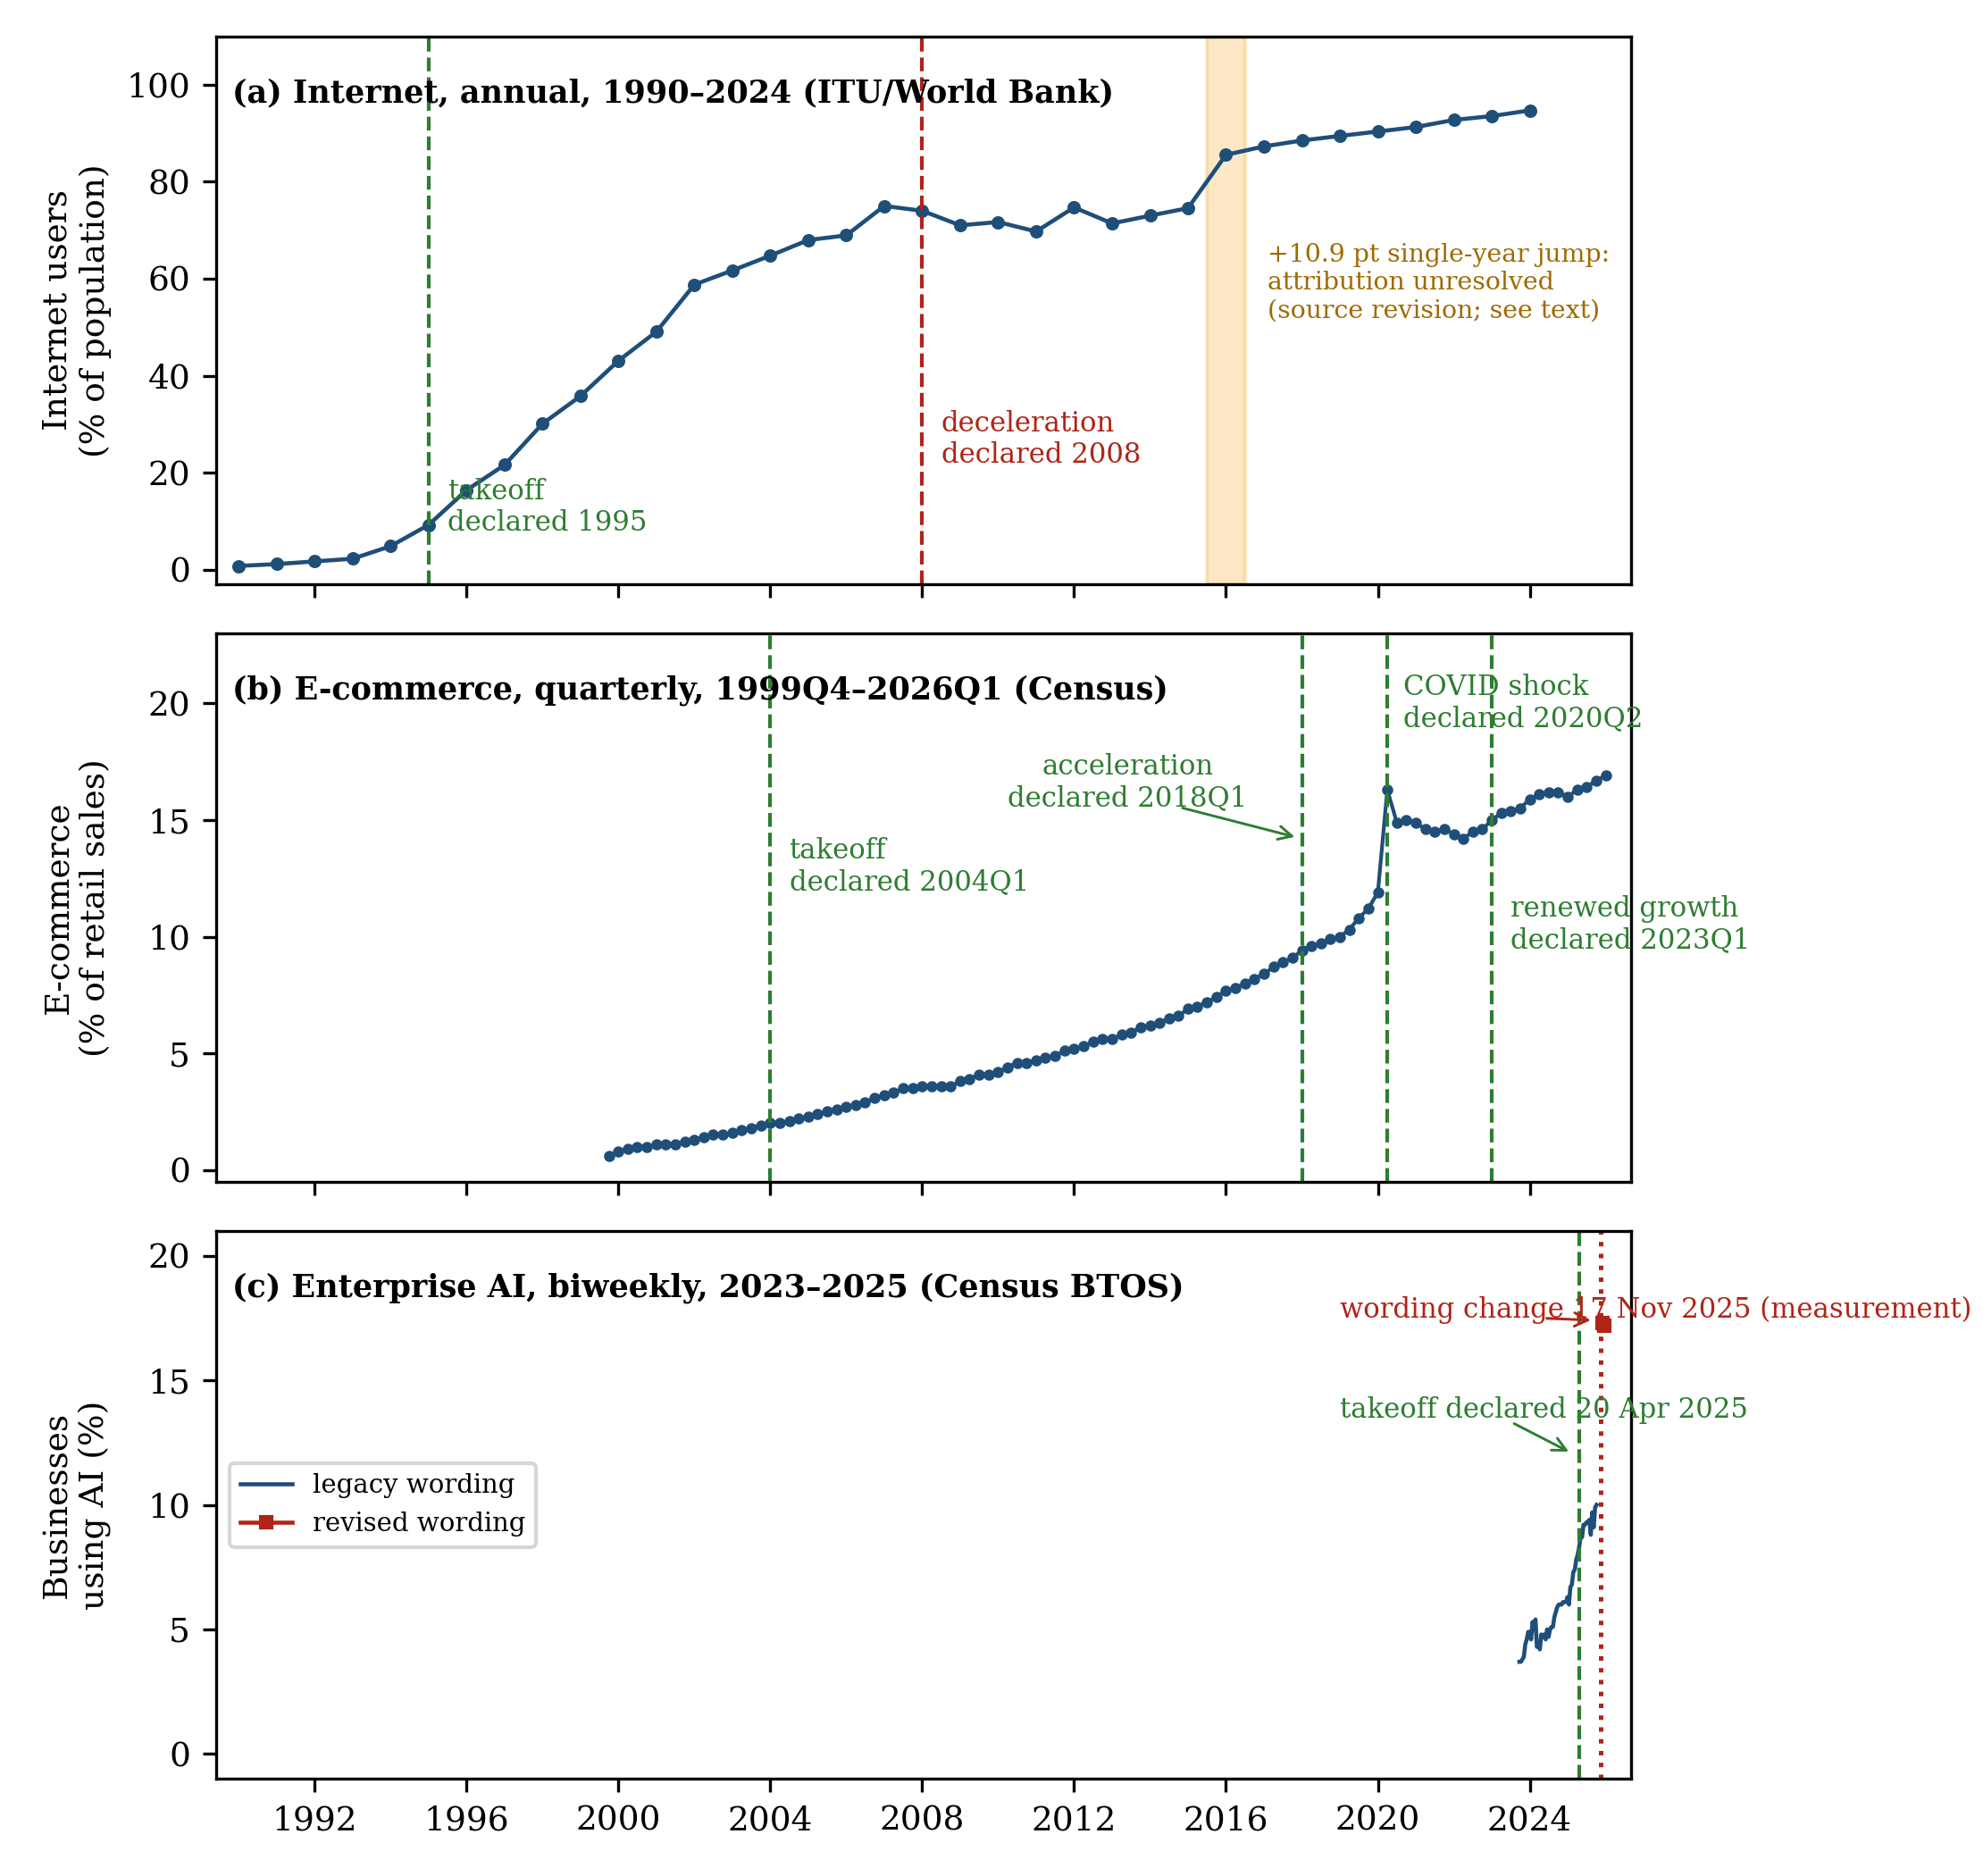
\includegraphics[width=0.98\textwidth]{figure6.png}
\caption{Three decades of U.S.\ digital technology diffusion under anytime-valid surveillance. (a) Internet users as a share of population, annual (ITU/World Bank via FRED); (b) e-commerce share of retail sales, quarterly (Census via FRED); (c) enterprise AI use, biweekly (Census BTOS; this paper's core application). Green dashed lines mark declared regime shifts; the red dashed line in (a) marks the declared deceleration; the red dotted line in (c) marks the excluded measurement intervention; the shaded band in (a) marks the 2016 single-year discontinuity whose attribution the available metadata cannot settle. Panels (a) and (b) use the plug-in-variance monitor of Section~\ref{sec:plugin}; panel (c) uses the exact design-based monitor.}
\label{fig:longview}
\end{figure}

\begin{table}[t]
\centering
\caption{Declared regime shifts across three diffusion waves, 1990--2026. The internet and e-commerce rows use the plug-in-variance monitor (approximate validity; Section~\ref{sec:plugin}); the enterprise-AI rows use the exact design-based monitor. Baseline slopes are in percentage points per period of the respective series (year, quarter, biweekly wave). E-values above $10^4$ are reported as decisive.}
\label{tab:longview}
\small
\begin{tabular}{lllr}
\toprule
Series and epoch baseline slope & Declared shift & Direction & Terminal $E$ \\
\midrule
\textit{Internet (annual)} & & & \\
\quad 0 (pre-registered) & 1995 & up (takeoff) & $>10^4$ \\
\quad $6.75$ (anchored 1996--2003) & 2008 & down (saturation onset) & 192.7 \\
\quad $1.46$ (anchored 2009--2016) & none by 2024 & --- & 0.7 \\
\addlinespace
\textit{E-commerce (quarterly)} & & & \\
\quad 0 (pre-registered) & 2004Q1 & up (takeoff) & 59.0 \\
\quad $0.10$ (anchored 2004--2006) & 2018Q1 & up (acceleration) & 52.4 \\
\quad $0.32$ (anchored 2018--2020) & 2020Q2 & up (COVID-19 shock) & $>10^4$ \\
\quad $-0.11$ (anchored 2020--2022) & 2023Q1 & up (renewed growth) & 79.1 \\
\quad $0.13$ (anchored 2023--2025) & none by 2026Q1 & --- & 1.3 \\
\addlinespace
\textit{Enterprise AI (biweekly)} & & & \\
\quad 0 (pre-registered) & 20 Apr 2025 & up (takeoff) & 42.2 \\
\quad $0.299$ (anchored Jan--Apr 2025) & none by Dec 2025 & (deceleration peaked at 24.3) & 4.5 \\
\bottomrule
\end{tabular}
\end{table}

Figure~\ref{fig:longview} and Table~\ref{tab:longview} place the AI episode in its evolutionary context. Run with the plug-in-variance monitor of Section~\ref{sec:plugin}, the surveillance recovers the punctuated record of U.S.\ digital diffusion as a sequence of dated declarations. For the internet, the takeoff is declared in 1995---the year commercial access became mainstream---against the pre-registered flat baseline; against the anchored boom-era growth rate of 6.75 points per year (1996--2003), the downward monitor declares the onset of saturation in 2008; and no further shift is declared through 2024 against the ensuing plateau-era baseline. For e-commerce the sequence is denser: takeoff declared in 2004Q1; a genuine acceleration in the growth \emph{rate}---from about 0.10 to about 0.32 points per quarter---declared in 2018Q1; the COVID-19 lockdown shock declared in the very quarter it occurred, 2020Q2, with decisive evidence; and, against the post-pandemic baseline of \emph{declining} share ($-0.11$ per quarter, anchored on 2020Q3--2022Q2), the resumption of growth declared in 2023Q1. The monitor is quiet where the series is quiet: no declaration stands open at the end of either sample.

Two lessons carry back to the paper's core argument. First, the COVID-19 episode furnishes the natural counterpart to the November 2025 BTOS redesign: both are large single-period jumps, but the 2020Q2 shock is a genuine diffusion event---externally corroborated, persistent in level, and occurring within an unchanged measurement instrument---whereas the 2025 jump is pure instrument. A monitoring architecture must be able to declare the first and absorb the second, and this one does. Second, the internet series contains the cautionary intermediate case: a $+10.9$-point jump in a single year (2015--2016) after a decade-long statistical plateau, a profile that under the diagnostic of Section~\ref{sec:diagnostic} is highly suspect as a measurement artifact---the series splices household-survey estimates with ITU and World Bank estimation methods \citep{fredinternet}---but that cannot be adjudicated, because no design-based errors, strata, or documented redesign dates accompany it. In our epoch structure the jump falls inside the 2009--2016 anchoring window and therefore contaminates the plateau-era baseline rather than triggering a declaration; an analyst without the measurement layer would have been left to guess. The comparison across the three panels of Figure~\ref{fig:longview} is thus also a comparison across measurement regimes---annual splices, quarterly designed surveys, biweekly designed surveys with published errors and strata---and it makes concrete how much inferential reach the improvement in measurement infrastructure has purchased.

\subsection{The intermediate waves: data mining, cloud, big data, data science, and deep learning}
\label{sec:waves}

\begin{figure}[t]
\centering
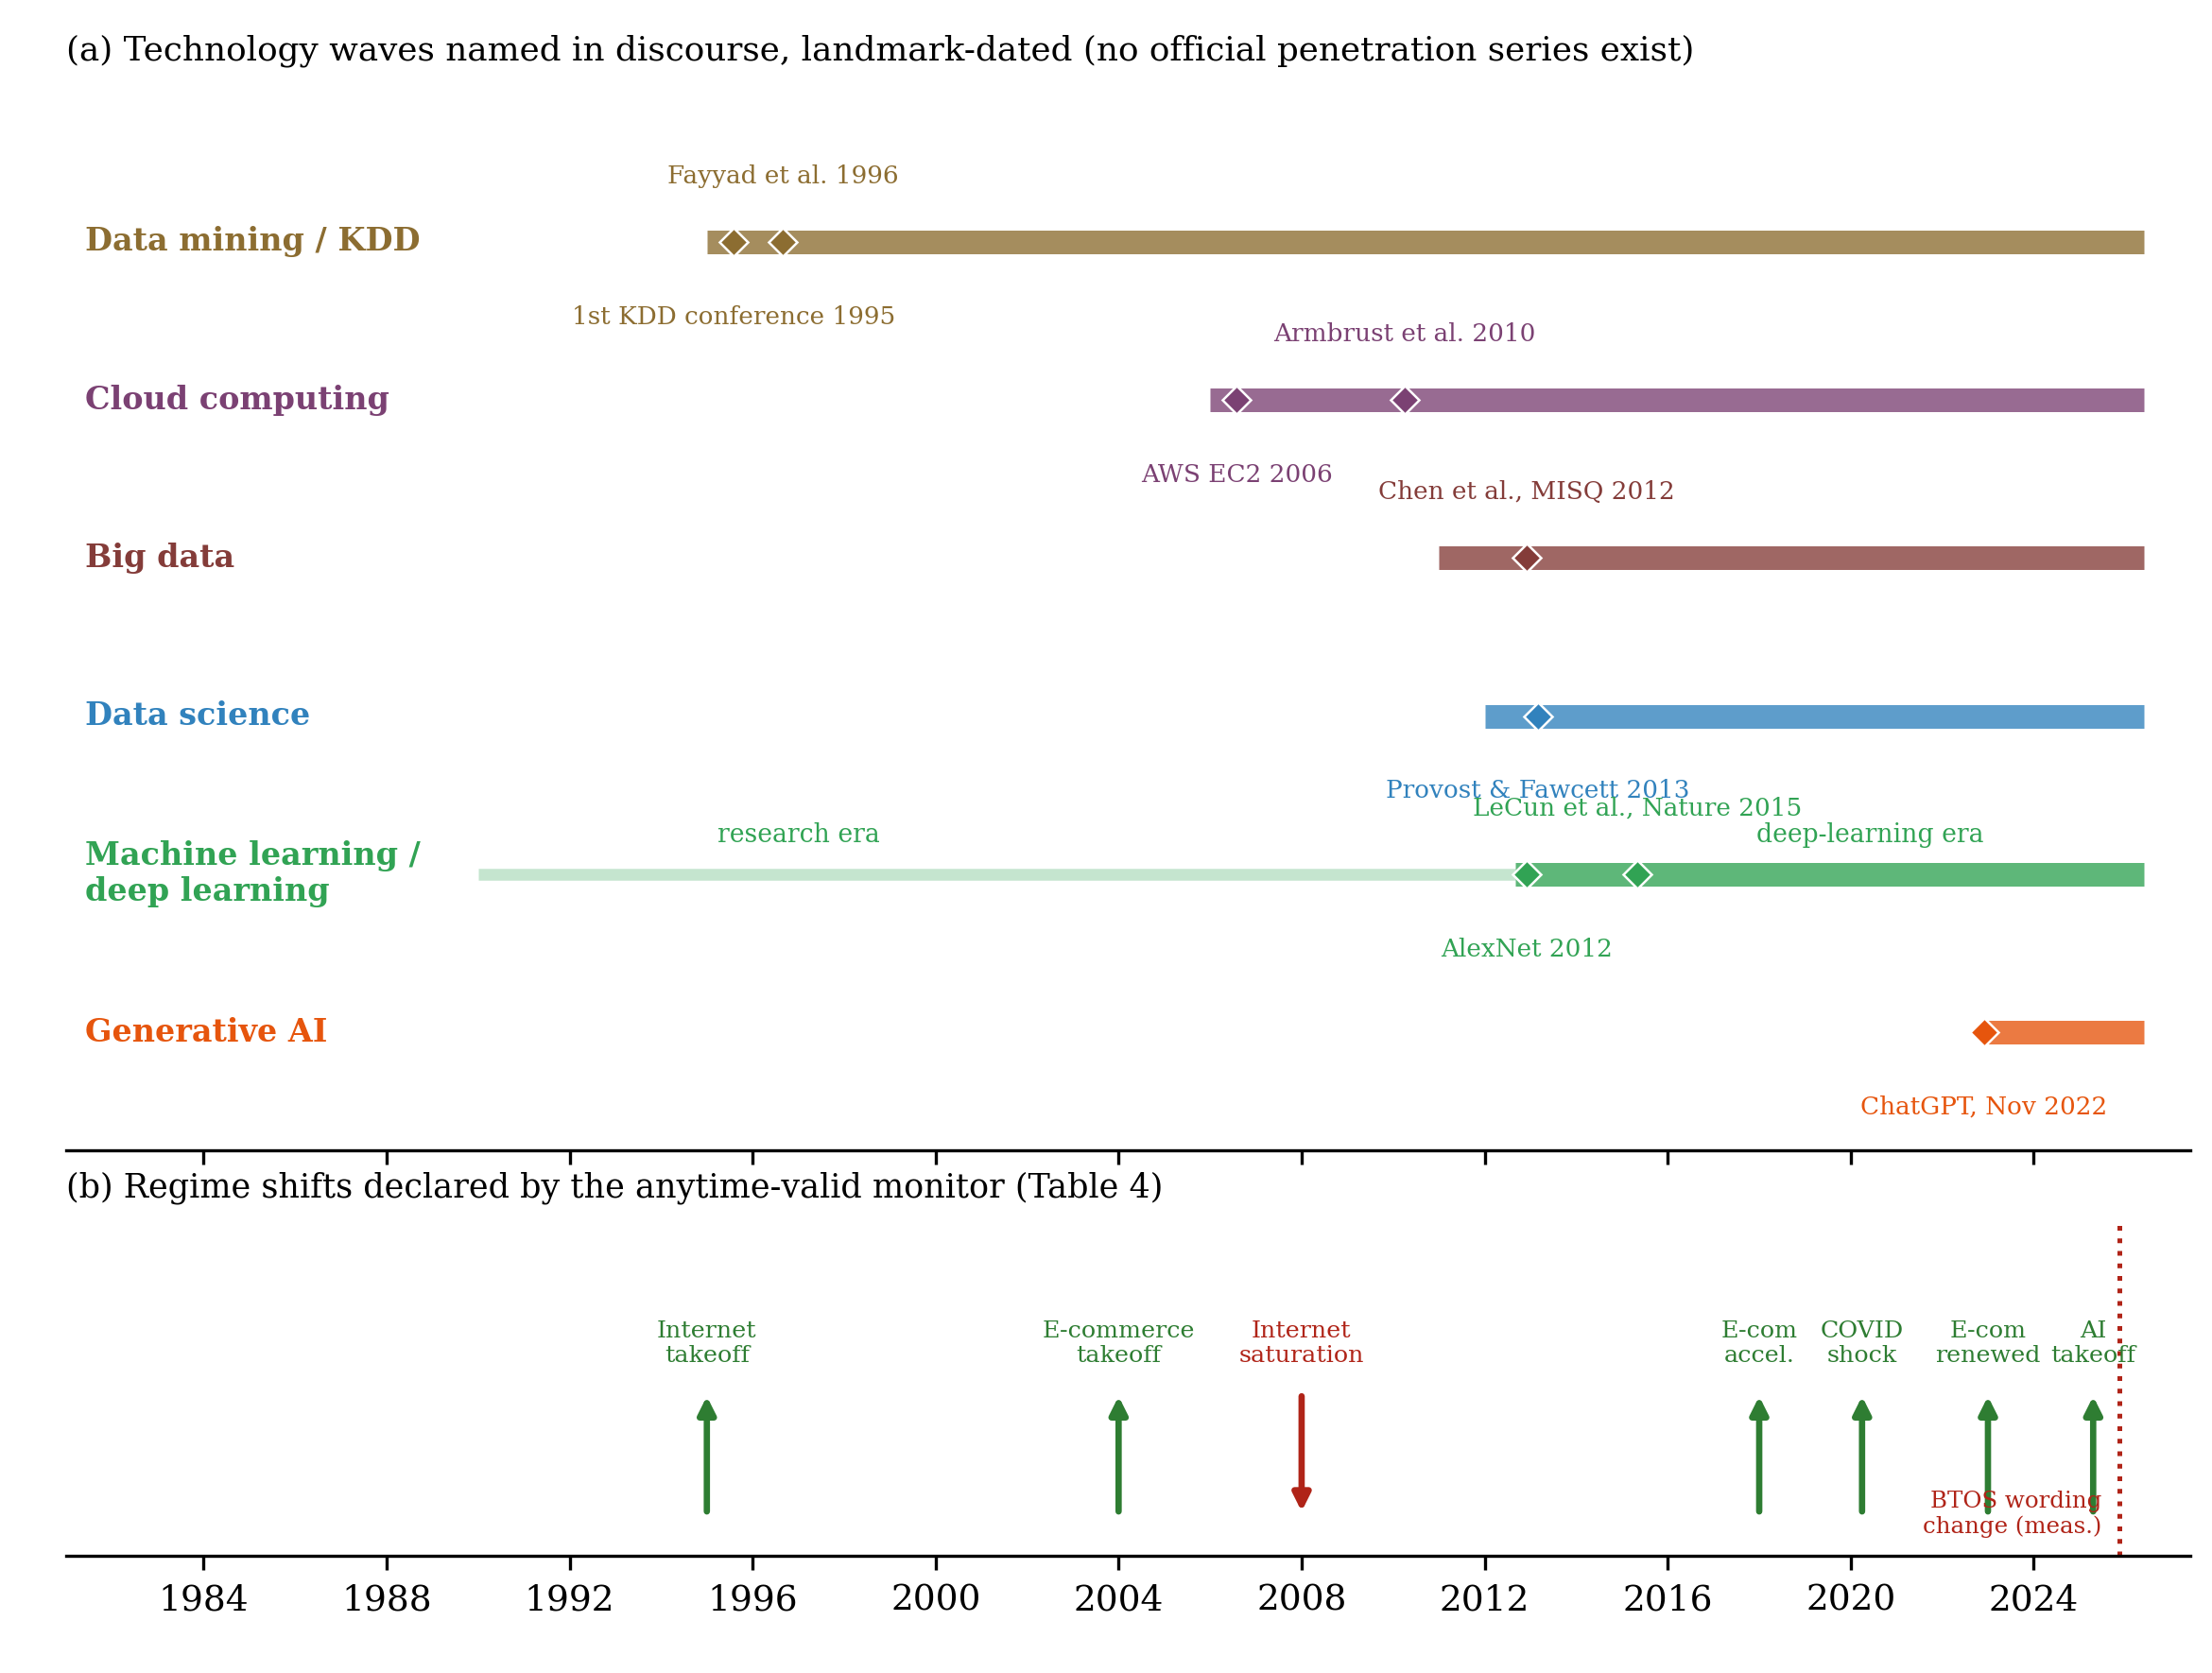
\includegraphics[width=0.98\textwidth]{figure7.png}
\caption{The technology waves of the analytics era, 1990--2026, aligned with the measured record. Panel (a) places the successive waves of technology discourse---data mining and knowledge discovery in databases \citep{fayyad1996}, cloud computing \citep{armbrust2010}, big data \citep{chen2012}, data science \citep{provost2013}, the deep-learning breakout within machine learning \citep{krizhevsky2017,lecun2015}, and generative AI---on a common timeline, each dated by canonical, citable landmarks (diamonds) rather than by penetration series, because no official adoption-share statistics were ever produced for these intermediate waves. Panel (b) repeats, on the same axis, the regime shifts declared by the anytime-valid monitor on the three measured series of Table~\ref{tab:longview}. Landmark dates: first ACM KDD conference (1995) and the KDD process framework \citep{fayyad1996}; Amazon EC2 launch (2006) and the Berkeley view of cloud computing \citep{armbrust2010}; the MIS Quarterly big-data agenda \citep{chen2012}; the codification of data science \citep{provost2013}; AlexNet \citep{krizhevsky2017} and the Nature review of deep learning \citep{lecun2015}; and the public release of ChatGPT (November 2022), the proximate trigger of the generative-AI wave \citep{bickblandin2025}.}
\label{fig:waves}
\end{figure}

Between the internet wave and the AI wave lie the technologies through which the analytics era actually arrived---data mining in the 1990s, cloud computing from 2006, big data and data science from the early 2010s, and the deep-learning breakout of 2012--2015. Figure~\ref{fig:waves} puts all of them in one picture, and it does so under an honesty constraint that is itself a finding: \emph{none} of these waves was ever tracked by an official penetration series. No statistical agency asked businesses, at any frequency, whether they used data mining in 1997, cloud infrastructure in 2009, or deep learning in 2016; the first designed, recurring, error-quantified adoption instrument for any of these general-purpose capabilities is the 2023 BTOS AI question set analyzed in this paper. The intermediate waves are therefore dated in panel (a) by canonical landmarks---the founding KDD conference and framework \citep{fayyad1996}, the EC2 launch and the Berkeley cloud retrospective \citep{armbrust2010}, the big-data research agenda \citep{chen2012}, the codification of data science \citep{provost2013}, AlexNet and the deep-learning consolidation \citep{krizhevsky2017,lecun2015}, and the ChatGPT release---rather than by measured curves, and we deliberately decline to substitute proxies such as search-interest or bibliometric indices for adoption shares within the monitoring framework, since their measurement processes (query-share renormalization, corpus growth, indexing-policy changes) are exactly the kind of undocumented instrument drift the framework exists to quarantine.

Read jointly, the two panels tell an evolutionary story with a measurement moral. The discourse waves cluster in the long gap between the internet's declared saturation onset (2008) and the AI takeoff (2025)---the period in which the capability stack (storage, elastic compute, learning algorithms) was assembled that the 2023--2025 AI diffusion then drew upon; the e-commerce acceleration declared in 2018Q1 is the one place where an intermediate wave leaves a footprint in a measured series, consistent with the maturation of cloud-era retail infrastructure in the mid-2010s. That the AI wave is the first to be observable biweekly, with design-based errors and strata, is why the monitoring guarantees of this paper became possible at all---and why, prospectively, the framework can be in place from a technology wave's first measured wave rather than reconstructed after the fact.

\subsection{Robustness}
\label{sec:robust}

Two sensitivity checks probe the construction. First, the prior scale: re-running the full surveillance with $\tau = 0.5$ and $\tau = 2$ leaves the takeoff declaration on 20 April 2025 for $\tau \in \{0.5, 1\}$ (terminal e-values 58.8 and 42.2) and moves it one wave later, to 4 May 2025, for $\tau = 2$ ($E = 45.8$); the qualitative Epoch-2 pattern is unchanged. Second, the sharp attribution of within-regime dispersion to sampling error: inflating every $\sigma_t$ by a factor $\kappa = 1.5$---equivalent to positing that half again as much wave-to-wave noise is non-informational---prevents any declaration in-sample (the takeoff monitor peaks at 5.8). The framework's conclusions are thus robust to the prior but, as they should be, sensitive to the variance model: the design-based standard errors are the published, defensible quantification of sampling noise for this survey, and analysts who believe substantial idiosyncratic latent wobble exists can encode that belief in $\kappa$ and accept correspondingly later detection. We regard the transparency of that dial as a feature: it makes explicit an assumption that rolling $t$-tests bury.

\section{Discussion}
\label{sec:discussion}

\subsection{Implications for technology and innovation management research}

Methodologically, the results argue that the arrival of streaming adoption data requires a matching change in inferential practice. Any TIM study that monitors an ongoing series---of adoption, patenting, platform activity---and reports significance at a data-dependent stopping point inherits the peeking problem, and Table~\ref{tab:methods} shows how badly it bites on real official data: even Bonferroni correction leaves a rule that alarms on nearly two-thirds of looks and certifies a survey redesign as the largest diffusion event on record. Anytime-valid tools remove the problem at negligible implementation cost---equation \eqref{eq:evalue} is one line---and change what a ``finding'' is: instead of a curve inflection estimated in hindsight, the analyst obtains a dated, auditable evidence trajectory recording exactly how much support a regime shift had at every moment. For the evolutionary perspective animating this special issue, that trajectory is the natural object: takeoffs, stalls, and punctuations become detected events with attached error guarantees, and the 2023--2025 history of enterprise AI---spurt, stall, sustained acceleration, plateau, resumption---is recovered here as precisely such a sequence.

Theoretically, treating measurement redesigns as causal interventions reframes the survey-comparability debate. The dispersion of AI adoption estimates across instruments \citep{crane2025} and the near-doubling of the BTOS measure under broader wording \citep{bick2026} are usually offered as reasons to distrust any single series. In our framework they are identified components of the observation function $g$ in \eqref{eq:obs}, and the November 2025 episode becomes a validation asset: a monitor that cannot absorb a known instrument intervention should not be trusted to interpret unknown ones. The cross-strata signature developed here---synchronization, extremity relative to each stratum's own history, mechanical sign coherence---gives applied researchers a portable screening rule for the redesigns that high-frequency programs will keep producing.

\subsection{Implications for practice}

For managers, the immediate application is internal. Enterprise AI deployments generate adoption telemetry---weekly active users, function-level usage, ticket volumes---that is reviewed continuously and acted upon under exactly the conditions that invalidate conventional tests. The protocol of Table~\ref{tab:protocol} transfers directly: define the baseline path for a pilot, run upward and downward monitors at a chosen $\alpha$, treat tool migrations and instrumentation changes as measurement interventions, and tie scale/hold/stop decisions to evidence thresholds. The Epoch-2 episode is the template for the hardest managerial call: when a promising deployment appears to stall, the monitor distinguishes ``24-to-1 evidence of a momentum break---prepare contingencies'' from ``regime change certified---act,'' and in this instance the distinction saved the (hypothetical) decision-maker from killing a trajectory that resumed within weeks. For analysts and policymakers consuming official statistics, the framework supplies a disciplined answer to the recurring question of whether the latest print signals genuine change, with error properties invariant to how often the question is asked.

\subsection{Limitations and future research}

Five limitations bound the claims. First, the public BTOS tabulations are aggregates from a rotating panel: the monitor tracks population-level rates, and firm-level regime dynamics---entry into and exit from AI use---are observable only through restricted microdata access, a natural Federal Statistical Research Data Center extension. Second, the adoption measure is a binary self-report; supplements measuring use across business functions \citep{census2026pr} invite multivariate e-processes over adoption depth, not just incidence. Third, the sharp null attributes all within-regime dispersion to design-based sampling error; the $\kappa$-robustness analysis shows detection timing depends materially on that attribution, and developing e-processes with data-driven yet valid overdispersion allowance is an open problem. Fourth, the attribution diagnostic for unannounced breaks is a screening rule with a causal rationale rather than an identified estimator; formal identification under richer instrument models would connect this work more deeply to the invariance literature. Fifth, the exact guarantees cover one technology in one country through December 2025, with only two post-redesign waves---too few to re-anchor the revised-regime monitor within sample; the 1990--2026 retrospective extends the surveillance logic across technologies but only with approximate, plug-in-variance validity and at coarse temporal resolution, so replications on the extending BTOS series, on the Eurostat enterprise ICT surveys, and on other economies' high-frequency programs remain the path to a comparative evolutionary evidence base with exact error control.

\section{Conclusion}
\label{sec:conclusion}

Technology adoption is now measured as a stream, but inference about it is still largely conducted as if data collection ended yesterday. This paper contributes a monitoring framework in which evidence about diffusion regime shifts is anytime-valid---robust to continuous inspection and optional stopping---and causally insulated from changes in the measurement apparatus itself. On the biweekly U.S.\ Census series for enterprise AI use, the framework declared the diffusion takeoff on 20 April 2025 at 42-to-1 evidence, held the mid-2025 deceleration at a peak of 24-to-1 without a false declaration, and absorbed a 26-standard-error survey redesign that conventional tests certify as the largest diffusion shock on record. Extended retrospectively across three decades, the same logic recovers the evolutionary record of U.S.\ digital diffusion---the internet's 1995 takeoff and 2008 saturation onset, e-commerce's 2004 takeoff, 2018 acceleration, 2020 pandemic shock, and 2023 re-acceleration---as a sequence of dated, directionally signed declarations, with the 2016 internet-series discontinuity standing as a reminder of what is lost when measurement travels without metadata. The broader proposal to the field is a change of stance: from fitting diffusion curves after the fact to running always-on, error-controlled surveillance of how social technologies evolve through the economy---and acting on that evidence with guarantees that survive the way evidence is actually consumed.

\section*{Declaration of competing interest}
The authors declare that they have no known competing financial interests or personal relationships that could have appeared to influence the work reported in this paper.

\section*{Data availability}
All data are public U.S.\ Census Bureau Business Trends and Outlook Survey statistics (\url{https://www.census.gov/hfp/btos/data_downloads}). The long-run series are retrieved from FRED: Internet users for the United States (ITNETUSERP2USA; \url{https://fred.stlouisfed.org/series/ITNETUSERP2USA}) and E-Commerce Retail Sales as a Percent of Total Sales (ECOMPCTSA; \url{https://fred.stlouisfed.org/series/ECOMPCTSA}). The exact analysis datasets (four CSV files: the spliced BTOS national and employment-size-class series with design-based standard errors and vintage provenance, and the two long-run series as retrieved) and replication scripts reproducing every number, table, and figure in the paper are provided as supplementary material.

\section*{Funding}
This research did not receive any specific grant from funding agencies in the public, commercial, or not-for-profit sectors.

\appendix

\section{The one-sided mixture e-process}
\label{app:derivation}

\paragraph{Derivation of \eqref{eq:evalue}.} Under $H_0^{(e)}$ in \eqref{eq:null}, the standardized increments $z_1, z_2, \dots$ are i.i.d.\ $\mathcal{N}(0,1)$. For a fixed drift $\delta$, the likelihood ratio of $\mathcal{N}(\delta,1)$ against $\mathcal{N}(0,1)$ after $n$ observations is $L_n(\delta) = \exp(\delta S_n - n\delta^2/2)$ with $S_n = \sum_{s \le n} z_s$, a nonnegative martingale with $L_0 = 1$. Mixing over the half-normal prior $\pi_\tau(\delta) = \frac{2}{\tau}\varphi(\delta/\tau)\mathbf{1}\{\delta > 0\}$ preserves the martingale property (Fubini), giving $E_n^{+} = \int_0^{\infty} L_n(\delta)\, \pi_\tau(\delta)\, d\delta$. Completing the square with $a_n = n + \tau^{-2}$,
\[
E_n^{+}
= \sqrt{\tfrac{2}{\pi\tau^2}} \int_0^{\infty} \exp\!\Big(-\tfrac{a_n}{2}\big(\delta - \tfrac{S_n}{a_n}\big)^2 + \tfrac{S_n^2}{2a_n}\Big) d\delta
= \frac{2}{\tau\sqrt{a_n}}\,\Phi\!\Big(\frac{S_n}{\sqrt{a_n}}\Big)\exp\!\Big(\frac{S_n^2}{2a_n}\Big),
\]
which is \eqref{eq:evalue}; at $n = 0$, $a_0 = \tau^{-2}$ and $E_0^{+} = 2\,\Phi(0) = 1$.

\paragraph{Validity under the composite one-sided null.} Suppose more generally that $z_t \mid \mathcal{F}_{t-1} \sim \mathcal{N}(\mu_t, 1)$ with $\mu_t \le 0$ (drift no greater than the baseline). For any $\delta > 0$, $\E[e^{\delta z_t - \delta^2/2} \mid \mathcal{F}_{t-1}] = e^{\delta \mu_t} \le 1$, so each $L_n(\delta)$ is a nonnegative supermartingale, and hence so is the mixture $E_n^{+}$. Ville's inequality for nonnegative supermartingales then gives $\Prob(\exists n: E_n^{+} \ge 1/\alpha') \le \alpha'$, establishing \eqref{eq:ville} with $\alpha' = \alpha/2$; the same argument applies to $E_n^{-}$ under $\mu_t \ge 0$, and running both monitors controls the per-epoch false-declaration probability at $\alpha$ by a union bound.

\section{Implementation parameters}
\label{app:implementation}

All computations use only information available at each wave, preserving predictability. Defaults: prior scale $\tau = 1$; level $\alpha = 0.05$ split equally across the two one-sided monitors (declaration threshold 40); anchoring window $w = 8$ waves with weighted-least-squares slope estimation (weights $1/\hat{\sigma}_t^2$) and the slope's standard error added to the increment variance as in \eqref{eq:null}; Epoch-1 baseline pre-registered at $\beta_1 = 0$; pre-announced instrument-transition increments excluded from all monitors. Comparators: two-sample $z$-tests on four-versus-four-wave windows using design-based standard errors, uncorrected at the two-sided 5\% level or Bonferroni-corrected by the running number of looks; moving-average rule with 3- and 8-wave windows. Retrospective (plug-in) runs: MAD window $W = 8$; floors $\phi = 0.8$ (internet, per year) and $\phi = 0.08$ (e-commerce, per quarter); residuals seeded from each anchoring window; e-values capped at $10^4$ for reporting. The replication scripts (\texttt{reproduce\_results.py} for the BTOS application; \texttt{reproduce\_retro.py} for the 1990--2026 retrospective) reproduce all reported values from the supplementary CSV files.

\bibliographystyle{elsarticle-harv}
\begin{thebibliography}{00}

\bibitem[{Armitage et~al.(1969)Armitage, McPherson and Rowe}]{armitage1969}
Armitage, P., McPherson, C.K., Rowe, B.C., 1969. Repeated significance tests on accumulating data. Journal of the Royal Statistical Society: Series A 132~(2), 235--244. \url{https://doi.org/10.2307/2343787}

\bibitem[{Armbrust et~al.(2010)Armbrust, Fox, Griffith, Joseph, Katz, Konwinski, Lee, Patterson, Rabkin, Stoica and Zaharia}]{armbrust2010}
Armbrust, M., Fox, A., Griffith, R., Joseph, A.D., Katz, R., Konwinski, A., Lee, G., Patterson, D., Rabkin, A., Stoica, I., Zaharia, M., 2010. A view of cloud computing. Communications of the ACM 53~(4), 50--58. \url{https://doi.org/10.1145/1721654.1721672}

\bibitem[{Bass(1969)}]{bass1969}
Bass, F.M., 1969. A new product growth model for consumer durables. Management Science 15~(5), 215--227. \url{https://doi.org/10.1287/mnsc.15.5.215}

\bibitem[{Bick(2026)}]{bick2026}
Bick, A., 2026. Measuring AI adoption among firms: How you ask matters. Federal Reserve Bank of St.\ Louis, On the Economy Blog, June 2026. \url{https://www.stlouisfed.org/on-the-economy/2026/jun/measuring-ai-adoption-firms-how-you-ask-matters}

\bibitem[{Bick et~al.(2025)Bick, Blandin and Deming}]{bickblandin2025}
Bick, A., Blandin, A., Deming, D.J., 2025. The rapid adoption of generative AI. NBER Working Paper No.\ 32966. National Bureau of Economic Research, Cambridge, MA. \url{https://doi.org/10.3386/w32966}

\bibitem[{Bonney et~al.(2024)Bonney, Breaux, Buffington, Dinlersoz, Foster, Goldschlag, Haltiwanger, Kroff and Savage}]{bonney2024}
Bonney, K., Breaux, C., Buffington, C., Dinlersoz, E., Foster, L., Goldschlag, N., Haltiwanger, J., Kroff, Z., Savage, K., 2024. Tracking firm use of AI in real time: A snapshot from the Business Trends and Outlook Survey. NBER Working Paper No.\ 32319. National Bureau of Economic Research, Cambridge, MA. \url{https://doi.org/10.3386/w32319}

\bibitem[{Chen et~al.(2012)Chen, Chiang and Storey}]{chen2012}
Chen, H., Chiang, R.H.L., Storey, V.C., 2012. Business intelligence and analytics: From big data to big impact. MIS Quarterly 36~(4), 1165--1188. \url{https://doi.org/10.2307/41703503}

\bibitem[{Crane et~al.(2025)Crane, Green and Soto}]{crane2025}
Crane, L., Green, M., Soto, P., 2025. Measuring AI uptake in the workplace. FEDS Notes, February 5, 2025. Board of Governors of the Federal Reserve System, Washington, DC. \url{https://doi.org/10.17016/2380-7172.3724}

\bibitem[{Davis(1989)}]{davis1989}
Davis, F.D., 1989. Perceived usefulness, perceived ease of use, and user acceptance of information technology. MIS Quarterly 13~(3), 319--340. \url{https://doi.org/10.2307/249008}

\bibitem[{Fayyad et~al.(1996)Fayyad, Piatetsky-Shapiro and Smyth}]{fayyad1996}
Fayyad, U., Piatetsky-Shapiro, G., Smyth, P., 1996. From data mining to knowledge discovery in databases. AI Magazine 17~(3), 37--54. \url{https://doi.org/10.1609/aimag.v17i3.1230}

\bibitem[{Federal Reserve Board(2026)}]{fed2026}
Federal Reserve Board, 2026. Monitoring AI adoption in the U.S.\ economy. FEDS Notes, April 3, 2026. Board of Governors of the Federal Reserve System, Washington, DC. \url{https://www.federalreserve.gov/econres/notes/feds-notes/monitoring-ai-adoption-in-the-u-s-economy-20260403.html}

\bibitem[{Garcia~Luna(2026)}]{garcialuna2026}
Garcia~Luna, E., 2026. AI adoption in business grows steadily but unevenly. Federal Reserve Bank of Minneapolis, May 2026. \url{https://www.minneapolisfed.org/article/2026/ai-adoption-in-business-grows-steadily-but-unevenly}

\bibitem[{Geroski(2000)}]{geroski2000}
Geroski, P.A., 2000. Models of technology diffusion. Research Policy 29~(4--5), 603--625. \url{https://doi.org/10.1016/S0048-7333(99)00092-X}

\bibitem[{Goldschlag(2025)}]{goldschlag2025}
Goldschlag, N., 2025. How many businesses are using AI? Agglomerations, December 19, 2025. \url{https://agglomerations.substack.com/p/how-many-businesses-are-using-ai}

\bibitem[{Gr\"unwald et~al.(2024)Gr\"unwald, de~Heide and Koolen}]{grunwald2024}
Gr\"unwald, P., de~Heide, R., Koolen, W.M., 2024. Safe testing. Journal of the Royal Statistical Society: Series B 86~(5), 1091--1128. \url{https://doi.org/10.1093/jrsssb/qkae011}

\bibitem[{Howard et~al.(2021)Howard, Ramdas, McAuliffe and Sekhon}]{howard2021}
Howard, S.R., Ramdas, A., McAuliffe, J., Sekhon, J., 2021. Time-uniform, nonparametric, nonasymptotic confidence sequences. Annals of Statistics 49~(2), 1055--1080. \url{https://doi.org/10.1214/20-AOS1991}

\bibitem[{Johari et~al.(2022)Johari, Koomen, Pekelis and Walsh}]{johari2022}
Johari, R., Koomen, P., Pekelis, L., Walsh, D., 2022. Always valid inference: Continuous monitoring of A/B tests. Operations Research 70~(3), 1806--1821. \url{https://doi.org/10.1287/opre.2021.2135}

\bibitem[{Krizhevsky et~al.(2017)Krizhevsky, Sutskever and Hinton}]{krizhevsky2017}
Krizhevsky, A., Sutskever, I., Hinton, G.E., 2017. ImageNet classification with deep convolutional neural networks. Communications of the ACM 60~(6), 84--90. \url{https://doi.org/10.1145/3065386}

\bibitem[{LeCun et~al.(2015)LeCun, Bengio and Hinton}]{lecun2015}
LeCun, Y., Bengio, Y., Hinton, G., 2015. Deep learning. Nature 521~(7553), 436--444. \url{https://doi.org/10.1038/nature14539}

\bibitem[{McElheran et~al.(2024)McElheran, Li, Brynjolfsson, Kroff, Dinlersoz, Foster and Zolas}]{mcelheran2024}
McElheran, K., Li, J.F., Brynjolfsson, E., Kroff, Z., Dinlersoz, E., Foster, L., Zolas, N., 2024. AI adoption in America: Who, what, and where. Journal of Economics \& Management Strategy 33~(2), 375--415. \url{https://doi.org/10.1111/jems.12576}

\bibitem[{Page(1954)}]{page1954}
Page, E.S., 1954. Continuous inspection schemes. Biometrika 41~(1--2), 100--115. \url{https://doi.org/10.1093/biomet/41.1-2.100}

\bibitem[{Pearl(2009)}]{pearl2009}
Pearl, J., 2009. Causality: Models, Reasoning, and Inference, second ed. Cambridge University Press, Cambridge. \url{https://doi.org/10.1017/CBO9780511803161}

\bibitem[{Peters et~al.(2016)Peters, B\"uhlmann and Meinshausen}]{peters2016}
Peters, J., B\"uhlmann, P., Meinshausen, N., 2016. Causal inference by using invariant prediction: Identification and confidence intervals. Journal of the Royal Statistical Society: Series B 78~(5), 947--1012. \url{https://doi.org/10.1111/rssb.12167}

\bibitem[{Provost and Fawcett(2013)}]{provost2013}
Provost, F., Fawcett, T., 2013. Data science and its relationship to big data and data-driven decision making. Big Data 1~(1), 51--59. \url{https://doi.org/10.1089/big.2013.1508}

\bibitem[{Ramdas et~al.(2023)Ramdas, Gr\"unwald, Vovk and Shafer}]{ramdas2023}
Ramdas, A., Gr\"unwald, P., Vovk, V., Shafer, G., 2023. Game-theoretic statistics and safe anytime-valid inference. Statistical Science 38~(4), 576--601. \url{https://doi.org/10.1214/23-STS894}

\bibitem[{Robbins(1970)}]{robbins1970}
Robbins, H., 1970. Statistical methods related to the law of the iterated logarithm. Annals of Mathematical Statistics 41~(5), 1397--1409. \url{https://doi.org/10.1214/aoms/1177696786}

\bibitem[{Rogers(2003)}]{rogers2003}
Rogers, E.M., 2003. Diffusion of Innovations, fifth ed. Free Press, New York. ISBN 9780743222099.

\bibitem[{Rothenh\"ausler et~al.(2021)Rothenh\"ausler, Meinshausen, B\"uhlmann and Peters}]{rothenhausler2021}
Rothenh\"ausler, D., Meinshausen, N., B\"uhlmann, P., Peters, J., 2021. Anchor regression: Heterogeneous data meet causality. Journal of the Royal Statistical Society: Series B 83~(2), 215--246. \url{https://doi.org/10.1111/rssb.12398}

\bibitem[{Shafer and Vovk(2019)}]{shafer2019}
Shafer, G., Vovk, V., 2019. Game-Theoretic Foundations for Probability and Finance. Wiley, Hoboken, NJ. \url{https://doi.org/10.1002/9781118548035}

\bibitem[{Shin et~al.(2023)Shin, Ramdas and Rinaldo}]{shin2023}
Shin, J., Ramdas, A., Rinaldo, A., 2023. E-detectors: A nonparametric framework for sequential change detection. The New England Journal of Statistics in Data Science 2~(2), 229--260. \url{https://doi.org/10.51387/23-NEJSDS51}

\bibitem[{U.S.~Census Bureau(2025)}]{censusmethod2025}
U.S.~Census Bureau, 2025. Business Trends and Outlook Survey: Methodology. U.S.\ Census Bureau, Washington, DC. \url{https://www2.census.gov/data/experimental-data-products/business-trends-and-outlook-survey/methodology.pdf}

\bibitem[{U.S.~Census Bureau(2026a)}]{censusstory2026}
U.S.~Census Bureau, 2026a. AI use at U.S.\ businesses. America Counts: Stories, May 26, 2026. \url{https://www.census.gov/library/stories/2026/05/ai-use-businesses.html}

\bibitem[{U.S.~Census Bureau(2026b)}]{census2026pr}
U.S.~Census Bureau, 2026b. Business Trends and Outlook Survey data release, May 7, 2026. Press release. \url{https://www.census.gov/newsroom/press-releases/2026/btos-may-7.html}

\bibitem[{U.S.~Census Bureau(2026c)}]{fredecom}
U.S.~Census Bureau, 2026c. E-commerce retail sales as a percent of total sales [ECOMPCTSA], seasonally adjusted, Q4 1999--Q1 2026. Retrieved from FRED, Federal Reserve Bank of St.\ Louis. \url{https://fred.stlouisfed.org/series/ECOMPCTSA}

\bibitem[{Vovk and Wang(2021)}]{vovk2021}
Vovk, V., Wang, R., 2021. E-values: Calibration, combination and applications. Annals of Statistics 49~(3), 1736--1754. \url{https://doi.org/10.1214/20-AOS2020}

\bibitem[{Wald(1945)}]{wald1945}
Wald, A., 1945. Sequential tests of statistical hypotheses. Annals of Mathematical Statistics 16~(2), 117--186. \url{https://doi.org/10.1214/aoms/1177731118}

\bibitem[{Waudby-Smith and Ramdas(2024)}]{waudbysmith2024}
Waudby-Smith, I., Ramdas, A., 2024. Estimating means of bounded random variables by betting. Journal of the Royal Statistical Society: Series B 86~(1), 1--27. \url{https://doi.org/10.1093/jrsssb/qkad009}

\bibitem[{World Bank(2026)}]{fredinternet}
World Bank, 2026. Internet users for the United States [ITNETUSERP2USA], annual, 1990--2024. Source: International Telecommunication Union, World Telecommunication/ICT Indicators database, and World Bank estimates. Retrieved from FRED, Federal Reserve Bank of St.\ Louis. \url{https://fred.stlouisfed.org/series/ITNETUSERP2USA}

\bibitem[{Zolas et~al.(2020)Zolas, Kroff, Brynjolfsson, McElheran, Beede, Buffington, Goldschlag, Foster and Dinlersoz}]{zolas2020}
Zolas, N., Kroff, Z., Brynjolfsson, E., McElheran, K., Beede, D., Buffington, C., Goldschlag, N., Foster, L., Dinlersoz, E., 2020. Advanced technologies adoption and use by U.S.\ firms: Evidence from the Annual Business Survey. NBER Working Paper No.\ 28290. National Bureau of Economic Research, Cambridge, MA. \url{https://doi.org/10.3386/w28290}

\end{thebibliography}

\end{document}
